\documentclass[11pt,a4paper]{article}
\usepackage[margin=2.4cm]{geometry}
\usepackage{amsmath,amssymb,booktabs}
\usepackage{tikz}
\usetikzlibrary{arrows.meta,positioning,calc,fit}
\usepackage[colorlinks=true,linkcolor=blue,citecolor=blue,urlcolor=blue]{hyperref}
\tikzset{
  box/.style={draw, rounded corners=1.5pt, align=left, text width=#1, inner sep=2.5pt, font=\footnotesize, fill=white},
  box/.default=9cm,
  dec/.style={box=#1, fill=blue!7, sharp corners},
  sr/.style={box=#1, fill=red!8},
  hl/.style={box=#1, fill=red!8, very thick},
  sw/.style={draw, dashed, align=left, text width=4.3cm, inner sep=2pt, font=\scriptsize, fill=yellow!15},
  arr/.style={-{Stealth[length=1.8mm]}, semithick},
}

\newcommand{\bA}{\mathbf A}
\newcommand{\bC}{\mathbf C}
\newcommand{\bK}{\mathbf K}
\newcommand{\bQ}{\mathbf Q}
\newcommand{\bG}{\mathbf G}
\newcommand{\bN}{\mathbf N}
\newcommand{\bW}{\mathbf W}
\newcommand{\bx}{\mathbf x}
\newcommand{\by}{\mathbf y}
\newcommand{\bz}{\mathbf z}
\newcommand{\bt}{\mathbf t}
\newcommand{\bb}{\mathbf b}
\newcommand{\bc}{\mathbf c}
\newcommand{\bd}{\mathbf d}
\newcommand{\bu}{\mathbf u}
\newcommand{\bv}{\mathbf v}
\newcommand{\code}[1]{\texttt{#1}}
\newcommand{\Tr}{\operatorname{Tr}}
\newcommand{\Sym}{\operatorname{Sym}}

\title{Algorithms and changes in FOCEX 9.0--9.9}
\author{K. Esfarjani}
\date{November 2026}

\begin{document}
\sloppy
\emergencystretch=3em
\maketitle

\begin{abstract}
FOCEX extracts force constants (FCs) of ranks 1 to 8 from force--displacement data of density-functional
calculations. Between 23 October and 6 November 2026 the code went from version 9.0 to
9.9. This paper documents, for developers and researchers, the problem behind each change, the
mathematics of the algorithm, and where it sits in the code, together with the tests that were run.
The main items are: invariance rows of all ranks from one loop; symmetry checks and symmetrization of the
structure, the Born charges and the stress; generalized Huang rows for a stressed reference;
Born--Huang elastic constants, $B_0'$ from FC3 and a rewritten quasi-harmonic model; mode Gr\"uneisen
parameters with an exact long-wave limit; standard errors of the FCs; relaxation of an unrelaxed
reference, with the full Ewald energy for point charges; IR/Raman activity from computed character
tables; partial refits with some ranks read; a hybrid Coulomb subtraction; elastic constants from the
long-wave sound speeds; an irreducible wedge from the Laue group; OpenMP; and a constrained LASSO with
exact invariances. Version 9.9 adds standard errors for LASSO fits, a noise test for the LASSO weight,
the smooth SVD filter written as a per-mode quadratic penalty, an optional ridge prior, a rule that moves
the SVD cut into a gap of the singular values, a refit when the measured noise exceeds the guess, and
rotational invariants of FC3 and FC4. A Wigner--Seitz boundary aliasing case that motivated the gap rule
is analysed, and a study of MoTe$_2$ shows how exact invariances distort the fit when the model or the data
are inconsistent with them.
\end{abstract}

\tableofcontents

%==============================================================================
\section{Introduction}
%==============================================================================
FOCEX expands the potential energy of a crystal about a reference structure in the atomic
displacements $u_i^\alpha$ (atom $i$, Cartesian direction $\alpha$):
\begin{equation}
E=E_0+\sum_{i\alpha}\Pi_i^\alpha u_i^\alpha+\frac1{2!}\sum\Phi_{ij}^{\alpha\beta}u_i^\alpha u_j^\beta
+\frac1{3!}\sum\Psi_{ijk}^{\alpha\beta\gamma}u_i^\alpha u_j^\beta u_k^\gamma
+\frac1{4!}\sum\chi_{ijkl}^{\alpha\beta\gamma\delta}u_i^\alpha u_j^\beta u_k^\gamma u_l^\delta+\dots
\label{eq:taylor}
\end{equation}
$\Pi$ (FC1), $\Phi$ (FC2), $\Psi$ (FC3), $\chi$ (FC4) and the higher ranks up to FC8 are the force
constants. The force $F_i^\alpha=-\partial E/\partial u_i^\alpha$ is linear in the FCs. The space-group
symmetry reduces the FCs of each rank to a set of irreducible values; every FC is a linear combination of
them. Stacking the forces of all atoms in all snapshots gives the linear system
\begin{equation}
\bA\bx\approx\bb ,
\end{equation}
where $\bx$ ($n_x$ entries) are the irreducible FCs of all ranks fitted, $\bb$ ($N$ entries) are the DFT
forces, and $\bA$ ($N\times n_x$) holds the products of displacements.

The FCs must also satisfy linear invariance relations $\bC\bx=\bd$: translational invariance (the
acoustic sum rules) of every rank, rotational invariance coupling ranks $n$ and $n-1$, and the Huang
conditions on FC2. $\bd=0$ except where the reference is stressed or a Coulomb part was subtracted
(Sections~\ref{sec:huang} and~\ref{sec:hybrid}). The switch \code{enforce\_inv} (\code{structure.params}
line~5, fourth value) chooses how the two systems are combined:
\begin{itemize}
\item 0: the invariance rows are stacked with the force rows and the whole system is solved by SVD
(Figs.~\ref{fig:svdset}, \ref{fig:solve01});
\item 1: $\bx=\bx_p+\bK\by$, with $\bK$ an orthonormal basis of the kernel of $\bC$ and $\bx_p$ a
particular solution; then $\min_\by\|\bA\bK\by-(\bb-\bA\bx_p)\|$ by SVD (\code{fit\_kernel\_basis},
\code{constrained\_fit.f90}). The invariances hold exactly (Fig.~\ref{fig:solve01});
\item 2 and 3: a LASSO on $\bx$ inside the same affine space, without and with a least-squares refit on
the selected FCs (Section~\ref{sec:lasso}, Figs.~\ref{fig:lassoouter}, \ref{fig:lassoinner}).
\end{itemize}
The least-squares SVD fits (\code{svd\_ridge.f90:svd\_set}) use the regularized back-substitution of \code{svbksb},
Section~\ref{sec:filter}; the kernel of the invariance rows is found with a hard cut
(\code{kernel\_and\_particular}). The relative cut is $c=\epsilon_F^2$, with $\epsilon_F$ the force error of
\code{default.params} line~2 (default $10^{-5}$, so $c=10^{-10}$; \code{ios.f90}).
\code{default.params} has 7 lines, each with a comment after its value: symmetry tolerance, force error,
\code{icutoff} (range of the neighbour search), margin (smallest FC written), \code{relax\_ref} (line 5),
\code{lasso\_rule} (line 6) and the ridge-prior switch \code{lasso\_l2} (line 7). FOCEX reads only the first
number of each line; lines 5--7 are optional and only the value 1 switches them on.

This paper takes the changes in order of version. Each section has a Motivation, an Algorithm and an
Implementation part, and a Validation paragraph where tests were recorded. Version dates and contents are
those of the manual (\code{docs/source/runfocex.rst}, Version history), the git tags \code{focex-9.0} to
\code{focex-9.8}, and the developer notes (\code{CLAUDE.md} of the repository). Numbers are copied from
those notes, the session notes and the README files of \code{FOCEX/REFERENCE/exact\_model}; the 9.9
results of Sections~\ref{sec:noisecheck} and~\ref{sec:mote2} are from runs of the final 9.9 build on
6 November 2026. Version 9.9 (6 November 2026; \code{FOCEX/Makefile} \code{ver=9.9}, manual history entry
9.9) is to be tagged \code{focex-9.9}.

Many tests below use the \emph{exact model} of \code{FOCEX/REFERENCE/exact\_model}: an energy that is a
polynomial of degree 4 in the positions (pair, three-body and four-body terms in squared distances), so
FC1 to FC4 are known exactly and FC5 and higher vanish. Its reference is stressed. It is set up for
fluorite CaF$_2$, wurtzite ZnO and monoclinic HfO$_2$, with 100 snapshots each.

%==============================================================================
\section{Program flow of FOCEX 9.9}\label{sec:flow}
%==============================================================================
Figures~\ref{fig:main}--\ref{fig:solve01} show the program as it is coded in 9.9, with the routine names (file:routine)
in the boxes; they were drawn from the code, not from the manual. Figure~\ref{fig:main} is the main program
\code{focex.f90} in the order of its calls, with the input switches beside the step where each acts.
Figure~\ref{fig:setup} expands the setup: inputs, symmetry, neighbour shells, FC groups and the FC2 keep rule,
supercells and snapshots, and the Coulomb subtraction. Figure~\ref{fig:linsys} shows how the two linear systems are
built: the force rows $\bA\bx\approx\bb$ and the invariance rows $\bC\bx=\bd$, and, for \code{enforce\_inv}$\ge1$,
the kernel $\bK$ and the particular solution $\bx_p$. Figure~\ref{fig:solve01} shows the solver branches. The SVD
solver \code{svd\_set} that \code{enforce\_inv}=0 and 1 share is in Fig.~\ref{fig:svdset}; the LASSO branch
(\code{enforce\_inv}=2, 3) is in Figs.~\ref{fig:lassoouter} and~\ref{fig:lassoinner} (Section~\ref{sec:lasso}). How
to read the branches: with 0 the invariance rows are just more rows of one least-squares problem; with 1, 2 and 3
only the force rows are fitted, and the invariances are built in by writing $\bx=\bx_p+\bK\by$ before the fit.
The lattice-dynamics part (\code{set\_band\_structure}) is in Figs.~\ref{fig:ld} and~\ref{fig:mech}, the
relaxation in Fig.~\ref{fig:relax}.
%------------------------------------------------------------------------------
\begin{figure}[p]
\centering
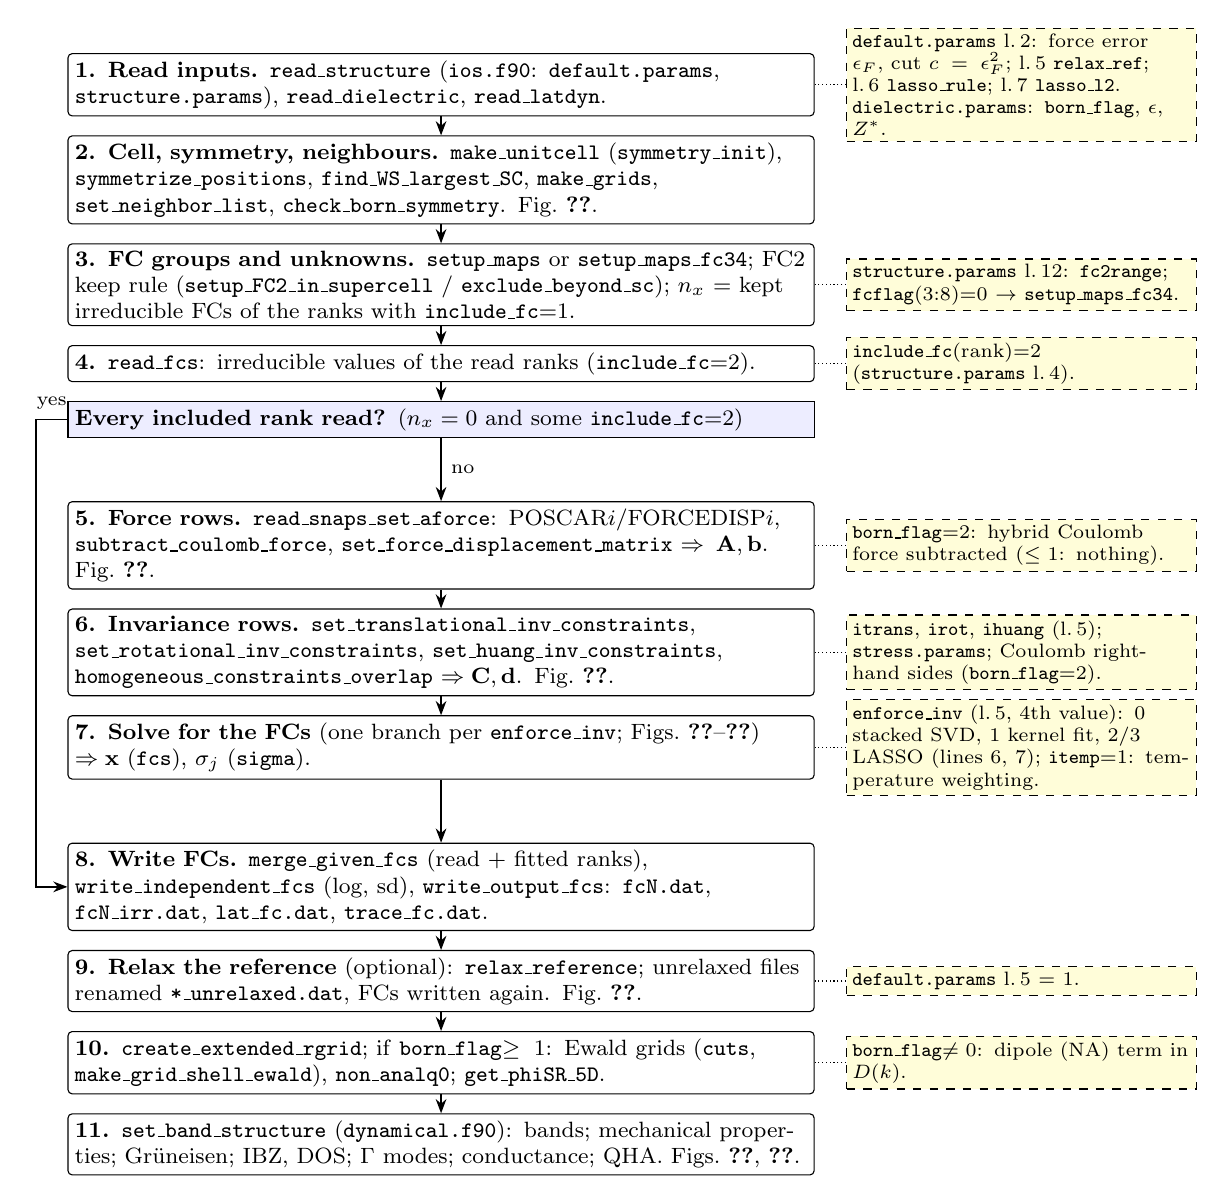
\begin{tikzpicture}[node distance=2.4mm]
\node[box=9.3cm] (a1) {\textbf{1. Read inputs.} \code{read\_structure} (\code{ios.f90}: \code{default.params}, \code{structure.params}),
  \code{read\_dielectric}, \code{read\_latdyn}.};
\node[box=9.3cm, below=of a1] (a2) {\textbf{2. Cell, symmetry, neighbours.} \code{make\_unitcell} (\code{symmetry\_init}),
  \code{symmetrize\_positions}, \code{find\_WS\_largest\_SC}, \code{make\_grids}, \code{set\_neighbor\_list},
  \code{check\_born\_symmetry}. Fig.~\ref{fig:setup}.};
\node[box=9.3cm, below=of a2] (a3) {\textbf{3. FC groups and unknowns.} \code{setup\_maps} or \code{setup\_maps\_fc34};
  FC2 keep rule (\code{setup\_FC2\_in\_supercell} / \code{exclude\_beyond\_sc}); $n_x$ = kept irreducible FCs of the
  ranks with \code{include\_fc}=1.};
\node[box=9.3cm, below=of a3] (a4) {\textbf{4.} \code{read\_fcs}: irreducible values of the read ranks (\code{include\_fc}=2).};
\node[dec=9.3cm, below=of a4] (d5) {\textbf{Every included rank read?} ($n_x=0$ and some \code{include\_fc}=2)};
\node[box=9.3cm, below=8mm of d5] (a6) {\textbf{5. Force rows.} \code{read\_snaps\_set\_aforce}: POSCAR$i$/FORCEDISP$i$,
  \code{subtract\_coulomb\_force}, \code{set\_force\_displacement\_matrix} $\Rightarrow \bA,\bb$. Fig.~\ref{fig:linsys}.};
\node[box=9.3cm, below=of a6] (a7) {\textbf{6. Invariance rows.} \code{set\_translational\_inv\_constraints},
  \code{set\_rotational\_inv\_constraints}, \code{set\_huang\_inv\_constraints}, \code{homogeneous\_constraints\_overlap}
  $\Rightarrow \bC,\bd$. Fig.~\ref{fig:linsys}.};
\node[box=9.3cm, below=of a7] (a8) {\textbf{7. Solve for the FCs} (one branch per \code{enforce\_inv}; Figs.~\ref{fig:svdset}--\ref{fig:lassoinner})
  $\Rightarrow \bx$ (\code{fcs}), $\sigma_j$ (\code{sigma}).};
\node[box=9.3cm, below=8mm of a8] (a9) {\textbf{8. Write FCs.} \code{merge\_given\_fcs} (read + fitted ranks),
  \code{write\_independent\_fcs} (log, sd), \code{write\_output\_fcs}: \code{fcN.dat}, \code{fcN\_irr.dat}, \code{lat\_fc.dat},
  \code{trace\_fc.dat}.};
\node[box=9.3cm, below=of a9] (a10) {\textbf{9. Relax the reference} (optional): \code{relax\_reference}; unrelaxed files renamed
  \code{*\_unrelaxed.dat}, FCs written again. Fig.~\ref{fig:relax}.};
\node[box=9.3cm, below=of a10] (a11) {\textbf{10.} \code{create\_extended\_rgrid}; if \code{born\_flag}$\ge1$: Ewald grids
  (\code{cuts}, \code{make\_grid\_shell\_ewald}), \code{non\_analq0}; \code{get\_phiSR\_5D}.};
\node[box=9.3cm, below=of a11] (a12) {\textbf{11.} \code{set\_band\_structure} (\code{dynamical.f90}): bands; mechanical properties;
  Gr\"uneisen; IBZ, DOS; $\Gamma$ modes; conductance; QHA. Figs.~\ref{fig:ld}, \ref{fig:mech}.};
\foreach \u/\v in {a1/a2,a2/a3,a3/a4,a4/d5,a6/a7,a7/a8,a9/a10,a10/a11,a11/a12} \draw[arr] (\u) -- (\v);
\draw[arr] (d5) -- node[right,font=\scriptsize]{no} (a6);
\draw[arr] (a8) -- (a9);
\draw[arr] (d5.west) -- ++(-4mm,0) node[above,font=\scriptsize,pos=0.5]{yes} |- (a9.west);
% switches
\node[sw, right=4mm of a1] (s1) {\code{default.params} l.\,2: force error $\epsilon_F$, cut $c=\epsilon_F^2$;
  l.\,5 \code{relax\_ref}; l.\,6 \code{lasso\_rule}; l.\,7 \code{lasso\_l2}. \code{dielectric.params}: \code{born\_flag}, $\epsilon$, $Z^*$.};
\node[sw, right=4mm of a3] (s3) {\code{structure.params} l.\,12: \code{fc2range}; \code{fcflag}(3:8)=0 $\to$ \code{setup\_maps\_fc34}.};
\node[sw, right=4mm of a4] (s4) {\code{include\_fc}(rank)=2 (\code{structure.params} l.\,4).};
\node[sw, right=4mm of a6] (s6) {\code{born\_flag}=2: hybrid Coulomb force subtracted ($\le1$: nothing).};
\node[sw, right=4mm of a7] (s7) {\code{itrans}, \code{irot}, \code{ihuang} (l.\,5); \code{stress.params}; Coulomb right-hand sides (\code{born\_flag}=2).};
\node[sw, right=4mm of a8] (s8) {\code{enforce\_inv} (l.\,5, 4th value): 0 stacked SVD, 1 kernel fit, 2/3 LASSO (lines 6, 7); \code{itemp}=1: temperature weighting.};
\node[sw, right=4mm of a10] (s10) {\code{default.params} l.\,5 = 1.};
\node[sw, right=4mm of a11] (s11) {\code{born\_flag}$\ne0$: dipole (NA) term in $D(k)$.};
\foreach \s/\t in {s1/a1,s3/a3,s4/a4,s6/a6,s7/a7,s8/a8,s10/a10,s11/a11} \draw[densely dotted] (\s.west) -- (\t.east);
\end{tikzpicture}
\caption{Main program \code{FOCEX/focex.f90} in the order of its calls. Dotted: the input switches that act at each
step (yellow). If every included rank is read, steps 5--7 are skipped (relax-only rerun, 9.8).}
\label{fig:main}
\end{figure}
%------------------------------------------------------------------------------
\begin{figure}[p]
\centering
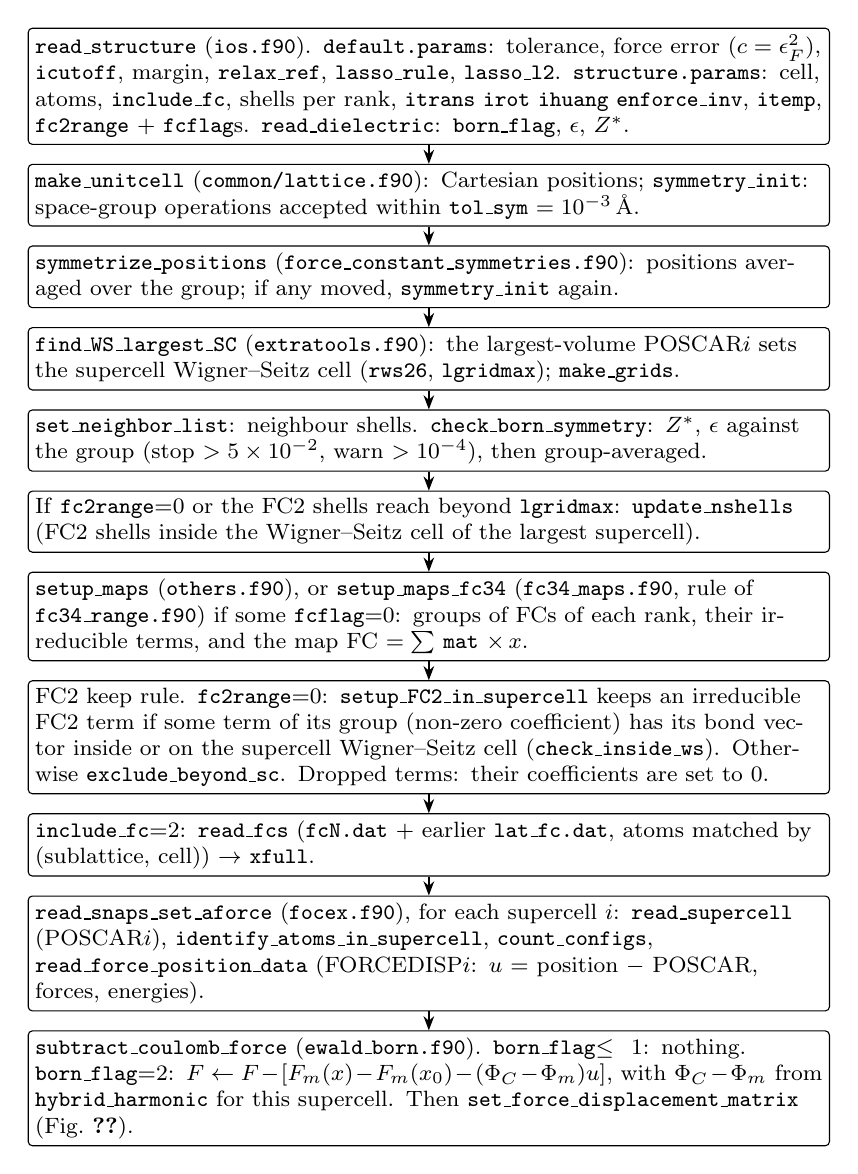
\begin{tikzpicture}[node distance=2.4mm]
\node[box=10cm] (b1) {\code{read\_structure} (\code{ios.f90}). \code{default.params}: tolerance, force error ($c=\epsilon_F^2$),
  \code{icutoff}, margin, \code{relax\_ref}, \code{lasso\_rule}, \code{lasso\_l2}. \code{structure.params}: cell, atoms,
  \code{include\_fc}, shells per rank, \code{itrans irot ihuang enforce\_inv}, \code{itemp}, \code{fc2range} + \code{fcflag}s.
  \code{read\_dielectric}: \code{born\_flag}, $\epsilon$, $Z^*$.};
\node[box=10cm, below=of b1] (b2) {\code{make\_unitcell} (\code{common/lattice.f90}): Cartesian positions;
  \code{symmetry\_init}: space-group operations accepted within \code{tol\_sym} $=10^{-3}$\,\AA.};
\node[box=10cm, below=of b2] (b3) {\code{symmetrize\_positions} (\code{force\_constant\_symmetries.f90}): positions averaged over the group;
  if any moved, \code{symmetry\_init} again.};
\node[box=10cm, below=of b3] (b4) {\code{find\_WS\_largest\_SC} (\code{extratools.f90}): the largest-volume POSCAR$i$ sets the supercell
  Wigner--Seitz cell (\code{rws26}, \code{lgridmax}); \code{make\_grids}.};
\node[box=10cm, below=of b4] (b5) {\code{set\_neighbor\_list}: neighbour shells. \code{check\_born\_symmetry}: $Z^*$, $\epsilon$ against the group
  (stop $>5\times10^{-2}$, warn $>10^{-4}$), then group-averaged.};
\node[box=10cm, below=of b5] (b6) {If \code{fc2range}=0 or the FC2 shells reach beyond \code{lgridmax}: \code{update\_nshells}
  (FC2 shells inside the Wigner--Seitz cell of the largest supercell).};
\node[box=10cm, below=of b6] (b7) {\code{setup\_maps} (\code{others.f90}), or \code{setup\_maps\_fc34} (\code{fc34\_maps.f90}, rule of
  \code{fc34\_range.f90}) if some \code{fcflag}=0: groups of FCs of each rank, their irreducible terms, and the map
  FC $=\sum$ \code{mat} $\times\,x$.};
\node[box=10cm, below=of b7] (b8) {FC2 keep rule. \code{fc2range}=0: \code{setup\_FC2\_in\_supercell} keeps an irreducible FC2 term if some term
  of its group (non-zero coefficient) has its bond vector inside or on the supercell Wigner--Seitz cell
  (\code{check\_inside\_ws}). Otherwise \code{exclude\_beyond\_sc}. Dropped terms: their coefficients are set to 0.};
\node[box=10cm, below=of b8] (b9) {\code{include\_fc}=2: \code{read\_fcs} (\code{fcN.dat} + earlier \code{lat\_fc.dat}, atoms matched by
  (sublattice, cell)) $\to$ \code{xfull}.};
\node[box=10cm, below=of b9] (b10) {\code{read\_snaps\_set\_aforce} (\code{focex.f90}), for each supercell $i$: \code{read\_supercell} (POSCAR$i$),
  \code{identify\_atoms\_in\_supercell}, \code{count\_configs}, \code{read\_force\_position\_data} (FORCEDISP$i$:
  $u$ = position $-$ POSCAR, forces, energies).};
\node[box=10cm, below=of b10] (b11) {\code{subtract\_coulomb\_force} (\code{ewald\_born.f90}). \code{born\_flag}$\le1$: nothing.
  \code{born\_flag}=2: $F\leftarrow F-[F_m(x)-F_m(x_0)-(\Phi_C-\Phi_m)u]$, with $\Phi_C-\Phi_m$ from \code{hybrid\_harmonic}
  for this supercell. Then \code{set\_force\_displacement\_matrix} (Fig.~\ref{fig:linsys}).};
\foreach \u/\v in {b1/b2,b2/b3,b3/b4,b4/b5,b5/b6,b6/b7,b7/b8,b8/b9,b9/b10,b10/b11} \draw[arr] (\u) -- (\v);
\end{tikzpicture}
\caption{Setup (steps 1--5 of Fig.~\ref{fig:main}). All routines are in \code{FOCEX/} unless a path is given. The
reading of \code{default.params} is part of \code{read\_structure}; there is no separate \code{read\_params}.}
\label{fig:setup}
\end{figure}
%------------------------------------------------------------------------------
\begin{figure}[p]
\centering
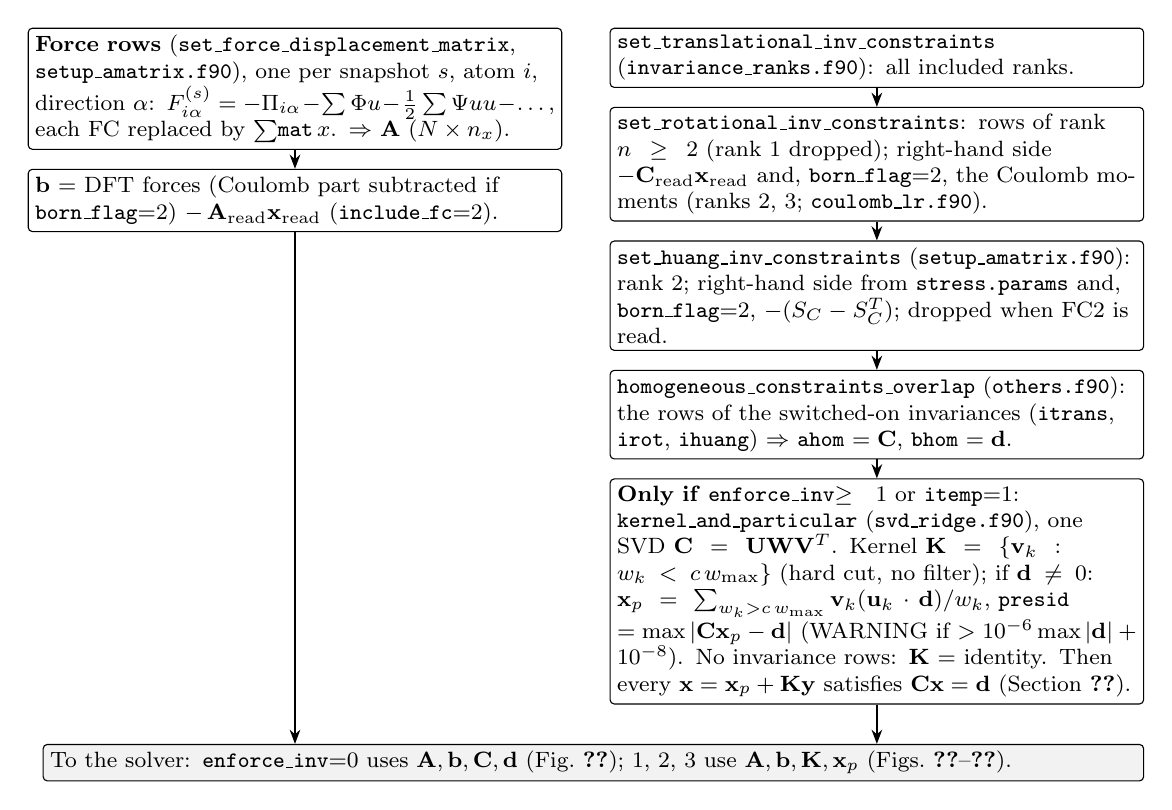
\begin{tikzpicture}[node distance=2.4mm]
\node[box=6.6cm] (c1) {\textbf{Force rows} (\code{set\_force\_displacement\_matrix}, \code{setup\_amatrix.f90}), one per snapshot
  $s$, atom $i$, direction $\alpha$:
  $F^{(s)}_{i\alpha}=-\Pi_{i\alpha}-\sum\Phi u-\tfrac12\sum\Psi uu-\dots$, each FC replaced by $\sum$\code{mat}$\,x$.
  $\Rightarrow$ $\bA$ ($N\times n_x$).};
\node[box=6.6cm, below=of c1] (c2) {$\bb$ = DFT forces (Coulomb part subtracted if \code{born\_flag}=2) $-\,\bA_{\rm read}\bx_{\rm read}$ (\code{include\_fc}=2).};
\node[box=6.6cm, right=6mm of c1.north east, anchor=north west] (c3) {\code{set\_translational\_inv\_constraints}
  (\code{invariance\_ranks.f90}): all included ranks.};
\node[box=6.6cm, below=of c3] (c4) {\code{set\_rotational\_inv\_constraints}: rows of rank $n\ge2$ (rank 1 dropped); right-hand side
  $-\bC_{\rm read}\bx_{\rm read}$ and, \code{born\_flag}=2, the Coulomb moments (ranks 2, 3; \code{coulomb\_lr.f90}).};
\node[box=6.6cm, below=of c4] (c5) {\code{set\_huang\_inv\_constraints} (\code{setup\_amatrix.f90}): rank 2; right-hand side from
  \code{stress.params} and, \code{born\_flag}=2, $-(S_C-S_C^T)$; dropped when FC2 is read.};
\node[box=6.6cm, below=of c5] (c6) {\code{homogeneous\_constraints\_overlap} (\code{others.f90}): the rows of the switched-on
  invariances (\code{itrans}, \code{irot}, \code{ihuang}) $\Rightarrow$ \code{ahom} $=\bC$, \code{bhom} $=\bd$.};
\node[box=6.6cm, below=of c6] (c7) {\textbf{Only if} \code{enforce\_inv}$\ge1$ or \code{itemp}=1:
  \code{kernel\_and\_particular} (\code{svd\_ridge.f90}), one SVD $\bC=\mathbf U\bW\mathbf V^T$.
  Kernel $\bK=\{\bv_k:\ w_k<c\,w_{\max}\}$ (hard cut, no filter); if $\bd\ne0$:
  $\bx_p=\sum_{w_k>c\,w_{\max}}\bv_k(\bu_k\cdot\bd)/w_k$, \code{presid} $=\max|\bC\bx_p-\bd|$ (WARNING if
  $>10^{-6}\max|\bd|+10^{-8}$). No invariance rows: $\bK$ = identity.
  Then every $\bx=\bx_p+\bK\by$ satisfies $\bC\bx=\bd$ (Section~\ref{sec:inhom}).};
\node[box=13.8cm, below=5mm of c7.south east, anchor=north east, fill=gray!10] (c8) {To the solver: \code{enforce\_inv}=0 uses $\bA,\bb,\bC,\bd$ (Fig.~\ref{fig:solve01});
  1, 2, 3 use $\bA,\bb,\bK,\bx_p$ (Figs.~\ref{fig:solve01}--\ref{fig:lassoinner}).};
\draw[arr] (c1) -- (c2); \draw[arr] (c3) -- (c4); \draw[arr] (c4) -- (c5); \draw[arr] (c5) -- (c6);
\draw[arr] (c6) -- (c7);
\draw[arr] (c2.south) -- (c2 |- c8.north);
\draw[arr] (c7) -- (c7 |- c8.north);
\end{tikzpicture}
\caption{The linear system: force rows $\bA\bx\approx\bb$ (left) and invariance rows $\bC\bx=\bd$ (right).}
\label{fig:linsys}
\end{figure}
%------------------------------------------------------------------------------
\begin{figure}[tbp]
\centering
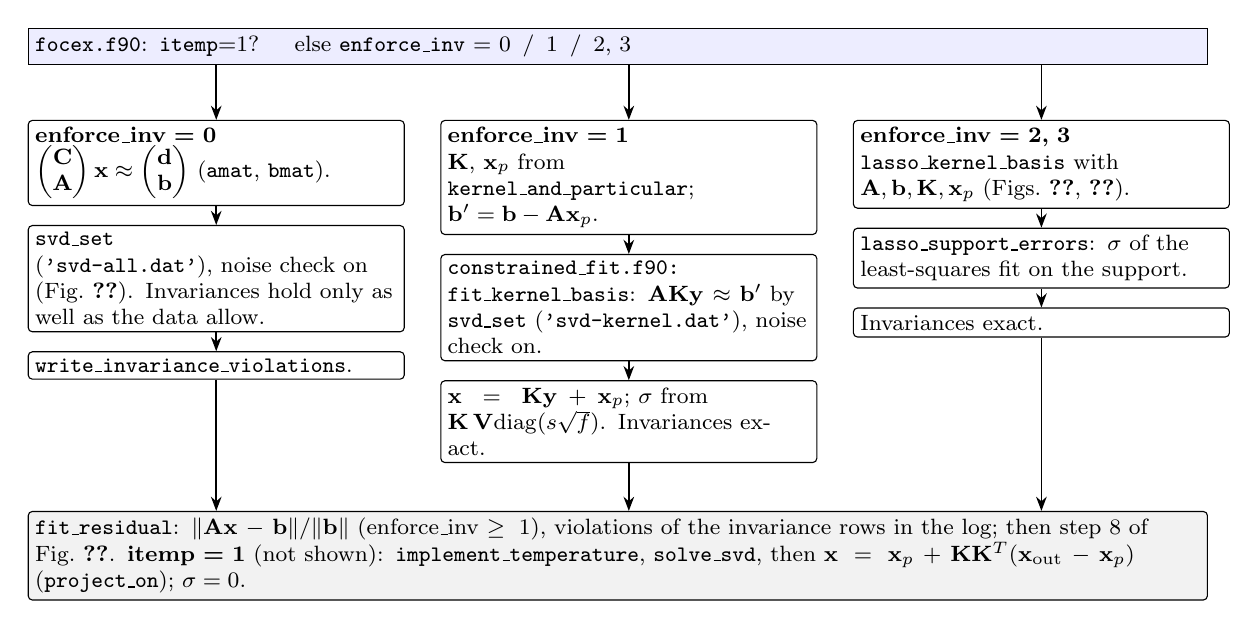
\begin{tikzpicture}[node distance=2.4mm]
\node[dec=14.8cm] (t) {\code{focex.f90}: \code{itemp}=1? \quad else \code{enforce\_inv} = 0 \,/\, 1 \,/\, 2, 3};
\node[box=4.6cm, below=7mm of t.south west, anchor=north west] (z1) {\textbf{enforce\_inv = 0}\\
  $\begin{pmatrix}\bC\\ \bA\end{pmatrix}\bx\approx\begin{pmatrix}\bd\\ \bb\end{pmatrix}$ (\code{amat}, \code{bmat}).};
\node[box=4.6cm, below=of z1] (z2) {\code{svd\_set}\\(\code{'svd-all.dat'}), noise check on (Fig.~\ref{fig:svdset}).
  Invariances hold only as well as the data allow.};
\node[box=4.6cm, below=of z2] (z3) {\code{write\_invariance\_violations}.};
\node[box=4.6cm, right=4.5mm of z1.north east, anchor=north west] (o1) {\textbf{enforce\_inv = 1}\\
  $\bK$, $\bx_p$ from \code{kernel\_and\_particular}; $\bb'=\bb-\bA\bx_p$.};
\node[box=4.6cm, below=of o1] (o2) {\code{constrained\_fit.f90:}\\\code{fit\_kernel\_basis}: $\bA\bK\by\approx\bb'$ by \code{svd\_set}
  (\code{'svd-kernel.dat'}), noise check on.};
\node[box=4.6cm, below=of o2] (o3) {$\bx=\bK\by+\bx_p$; $\sigma$ from $\bK\,\mathbf V\mathrm{diag}(s\sqrt f)$. Invariances exact.};
\node[box=4.6cm, right=4.5mm of o1.north east, anchor=north west] (l1) {\textbf{enforce\_inv = 2, 3}\\
  \code{lasso\_kernel\_basis} with $\bA,\bb,\bK,\bx_p$ (Figs.~\ref{fig:lassoouter}, \ref{fig:lassoinner}).};
\node[box=4.6cm, below=of l1] (l2) {\code{lasso\_support\_errors}: $\sigma$ of the least-squares fit on the support.};
\node[box=4.6cm, below=of l2] (l3) {Invariances exact.};
\node[fit=(z3)(o3)(l3),inner sep=0pt] (bot) {};
\node[box=14.8cm, anchor=north west, fill=gray!10] (f) at ([yshift=-6mm]bot.south -| z1.west) {\code{fit\_residual}: $\|\bA\bx-\bb\|/\|\bb\|$
  (enforce\_inv $\ge1$), violations of the invariance rows in the log; then step 8 of Fig.~\ref{fig:main}.
  \textbf{itemp = 1} (not shown): \code{implement\_temperature}, \code{solve\_svd}, then $\bx=\bx_p+\bK\bK^T(\bx_{\rm out}-\bx_p)$ (\code{project\_on}); $\sigma=0$.};
\draw[arr] (t.south -| z1) -- (z1); \draw[arr] (t.south -| o1) -- (o1); \draw[arr] (t.south -| l1) -- (l1);
\draw[arr] (z1)--(z2); \draw[arr] (z2)--(z3); \draw[arr] (o1)--(o2); \draw[arr] (o2)--(o3);
\draw[arr] (l1)--(l2); \draw[arr] (l2)--(l3);
\draw[arr] (z3) -- (z3 |- f.north); \draw[arr] (o3) -- (o3 |- f.north); \draw[arr] (l3) -- (l3 |- f.north);
\end{tikzpicture}
\caption{Solving for the FCs: the branches of \code{focex.f90} for \code{enforce\_inv}. Only the force rows enter the
fits of 1, 2 and 3; the invariances enter through $\bK$ and $\bx_p$.}
\label{fig:solve01}
\end{figure}
%------------------------------------------------------------------------------
\begin{figure}[tbp]
\centering
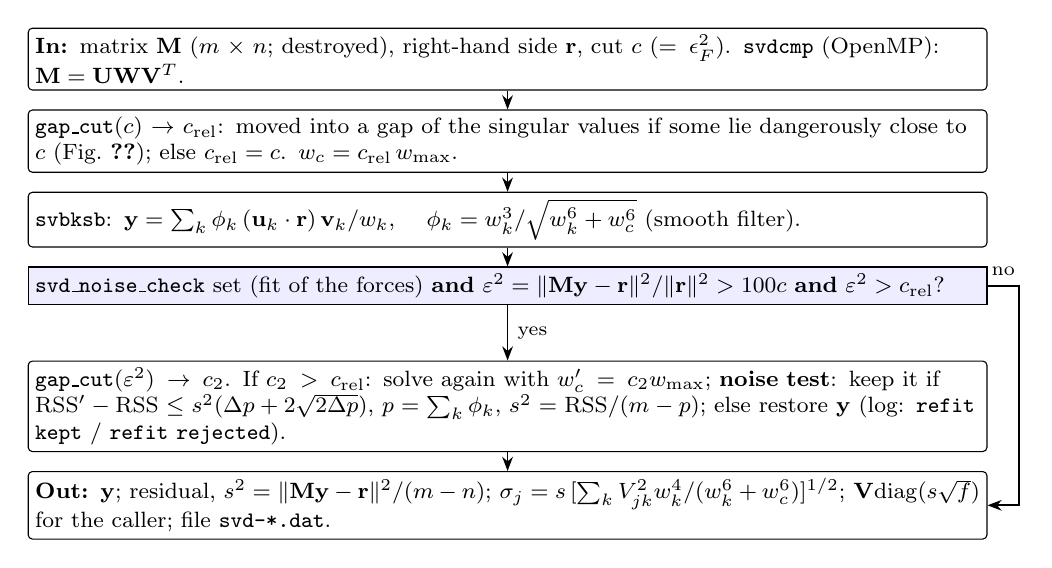
\begin{tikzpicture}[node distance=2.4mm]
\node[box=12cm] (e1) {\textbf{In:} matrix $\mathbf M$ ($m\times n$; destroyed), right-hand side $\mathbf r$, cut $c$ ($=\epsilon_F^2$).
  \code{svdcmp} (OpenMP): $\mathbf M=\mathbf U\bW\mathbf V^T$.};
\node[box=12cm, below=of e1] (e2) {\code{gap\_cut}$(c)\to c_{\rm rel}$: moved into a gap of the singular values if some lie
  dangerously close to $c$ (Fig.~\ref{fig:gap}); else $c_{\rm rel}=c$. $w_c=c_{\rm rel}\,w_{\max}$.};
\node[box=12cm, below=of e2] (e3) {\code{svbksb}: $\by=\sum_k\phi_k\,(\bu_k\cdot\mathbf r)\,\bv_k/w_k$, \quad
  $\phi_k=w_k^3/\sqrt{w_k^6+w_c^6}$ (smooth filter).};
\node[dec=12cm, below=of e3] (e4) {\code{svd\_noise\_check} set (fit of the forces) \textbf{and} $\varepsilon^2=\|\mathbf M\by-\mathbf r\|^2/\|\mathbf r\|^2>100c$
  \textbf{and} $\varepsilon^2>c_{\rm rel}$?};
\node[box=12cm, below=7mm of e4] (e5) {\code{gap\_cut}$(\varepsilon^2)\to c_2$. If $c_2>c_{\rm rel}$: solve again with $w_c'=c_2w_{\max}$;
  \textbf{noise test}: keep it if $\mathrm{RSS}'-\mathrm{RSS}\le s^2(\Delta p+2\sqrt{2\Delta p})$, $p=\sum_k\phi_k$,
  $s^2=\mathrm{RSS}/(m-p)$; else restore $\by$ (log: \code{refit kept} / \code{refit rejected}).};
\node[box=12cm, below=of e5] (e6) {\textbf{Out:} $\by$; residual, $s^2=\|\mathbf M\by-\mathbf r\|^2/(m-n)$;
  $\sigma_j=s\,[\sum_kV_{jk}^2w_k^4/(w_k^6+w_c^6)]^{1/2}$; $\mathbf V\mathrm{diag}(s\sqrt{f})$ for the caller; file \code{svd-*.dat}.};
\draw[arr] (e1) -- (e2); \draw[arr] (e2) -- (e3); \draw[arr] (e3) -- (e4);
\draw[arr] (e4) -- node[right,font=\scriptsize]{yes} (e5); \draw[arr] (e5) -- (e6);
\draw[arr] (e4.east) -- ++(4mm,0) node[above,font=\scriptsize,pos=0.5]{no} |- (e6.east);
\end{tikzpicture}
\caption{\code{svd\_ridge.f90:svd\_set}, the SVD solver of \code{enforce\_inv}=0 and 1 (and of
\code{lasso\_support\_errors}, with \code{svd\_noise\_check} off).}
\label{fig:svdset}
\end{figure}

%==============================================================================
\section{Homogeneous and inhomogeneous rows}\label{sec:inhom}
%==============================================================================
\paragraph{Design.} The linear system has a homogeneous part, the invariance rows with right-hand side 0, and an
inhomogeneous part: the force rows, and every invariance row that has a right-hand side. The invariance rows of
both kinds are exact constraints; only the force rows are fitted by least squares.

\paragraph{How a row becomes inhomogeneous} (read in the code):
\begin{enumerate}
\item \code{include\_fc}(r)=2. The read FCs are not unknowns. Their contribution moves to the right-hand side of the
force rows (\code{setup\_amatrix.f90:set\_force\_displacement\_matrix}, lines 223--226:
$b\leftarrow b-u\,\mathrm{mat}\,x_{\rm read}$) and of every translational and rotational row that contains rank $r$
(\code{invariance\_ranks.f90}: a read term gets column $-1$, and \code{gather\_rows} sums those contributions into the
row's right-hand side, near line 304). A row with no fitted column left is dropped, and the largest residual of the
read FCs in such rows is logged.
\item A stressed reference (\code{stress.params}). The Huang rows get the right-hand side
$-2\Omega(\delta_{\alpha\beta}\sigma_{\gamma\delta}-\delta_{\gamma\delta}\sigma_{\alpha\beta})$, $\Omega$ the volume of the primitive cell
(\code{setup\_amatrix.f90:set\_huang\_inv\_constraints}, lines 125--126; the stress is point-group averaged there first).
Huang rows exist only when FC2 is fitted (\code{include\_fc}(2)=1).
\item \code{born\_flag}=2. Rank-2 rotational rows get $-\sum_{a\mu}M(i_1;\alpha_1,a,\mu)\varepsilon_{a\mu\nu}$ from \code{lr\_moments};
rank-3 rows get the \code{lr\_rot3\_pair} / \code{lr\_rot3\_onsite} terms
(\code{invariance\_ranks.f90:set\_rotational\_inv\_constraints}, lines 188--233). The Huang right-hand side is corrected by
$-(S_C-S_C^T)$. Translational rows stay homogeneous: the subtracted harmonic Coulomb part obeys the sum rule in the
supercell. Rotational rows of rank $\ge4$ get no Coulomb right-hand side (open point for anisotropic $Z^*$).
\end{enumerate}

\begin{table}[htbp]
\centering
\caption{Right-hand side $d$ of each kind of invariance row. ``0'': the row is homogeneous in that case.}
\label{tab:inhom}
\small
\begin{tabular}{@{}p{2.9cm}p{3.6cm}p{3.1cm}p{4.2cm}@{}}
\toprule
row & \code{include\_fc}(r)=2 & \code{stress.params} & \code{born\_flag}=2\\
\midrule
translational, rank $n$ & $-\bC_{\rm read}\bx_{\rm read}$ if $r=n$ & 0 & 0\\
rotational, rank $n$ & $-\bC_{\rm read}\bx_{\rm read}$ if $r\in\{n-1,n\}$ & 0 & $n=2$: $-M\!:\!\varepsilon$; $n=3$: \code{lr\_rot3}; $n\ge4$: 0\\
Huang (rank 2) & no rows if $r=2$ & $-2\Omega(\delta\sigma-\delta\sigma)$ & $-(S_C-S_C^T)$\\
force rows & $\bb-\bA_{\rm read}\bx_{\rm read}$ & $\bb$ & $\bb$ minus the Coulomb force\\
\bottomrule
\end{tabular}
\end{table}

\paragraph{How the code solves it.} All invariance rows, homogeneous or not, are kept in one matrix \code{ahom} with
right-hand side \code{bhom} (\code{others.f90:homogeneous\_constraints\_overlap}). One SVD of \code{ahom}
(\code{svd\_ridge.f90:kernel\_and\_particular}) gives the kernel $\bK$ and, only when some \code{bhom} $\ne0$, the
particular solution $\bx_p$; every $\bx=\bx_p+\bK\by$ satisfies all invariance rows exactly. This is the two-part
design as long as the inhomogeneous invariance rows remain exact constraints, which they do: they are not moved into
the least-squares block. The solvers then use it as follows (Fig.~\ref{fig:inhom}):
\code{enforce\_inv}=1 fits $\bb-\bA\bx_p$ in $\bK$ and returns $\bx=\bx_p+\bK\by$; 2 and 3 pass $\bx_0=\bx_p$ to the LASSO
($\bz_0=\bW\bx_0$, and \code{refit\_support} keeps $(\bz_0+\bQ\bt)_j=0$ off the support through its \code{shift\_part});
0 stacks $[\code{ahom};\code{aforce}]$ with $[\code{bhom};\code{bforce}]$, so that there all rows, homogeneous or not,
are fitted together. Since the audit of 6 November 2026 (Section~\ref{sec:audit}) a WARNING is printed when
$\max|\bC\bx_p-\bd|>10^{-6}\max|\bd|+10^{-8}$: inconsistent inhomogeneous rows (read FCs, stress or Coulomb terms that
contradict the other rows).

\begin{figure}[htbp]
\centering
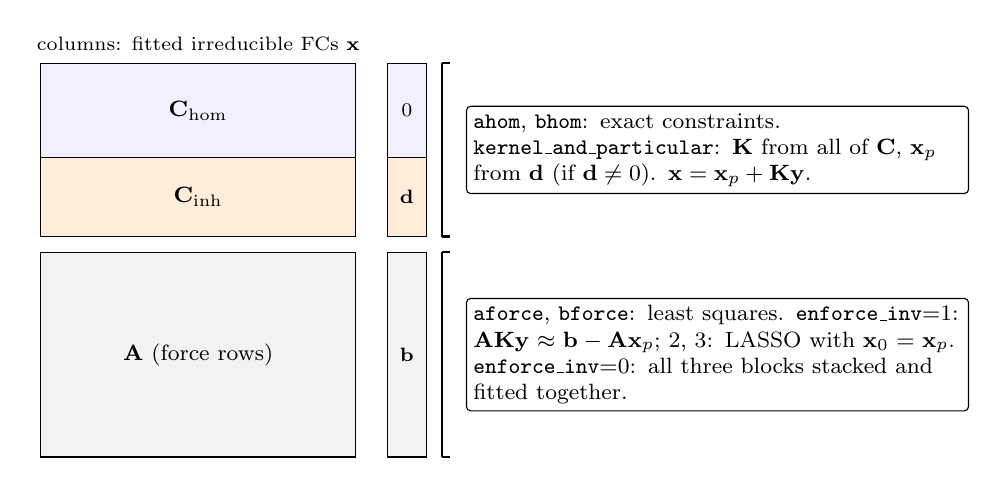
\begin{tikzpicture}
\draw[fill=blue!6] (0,2.2) rectangle (4,3.4); \node[font=\footnotesize,align=center] at (2,2.8) {$\bC_{\rm hom}$};
\draw[fill=orange!15] (0,1.2) rectangle (4,2.2); \node[font=\footnotesize,align=center] at (2,1.7) {$\bC_{\rm inh}$};
\draw[fill=gray!10] (0,-1.6) rectangle (4,1.0); \node[font=\footnotesize] at (2,-0.3) {$\bA$ (force rows)};
\draw[fill=blue!6] (4.4,2.2) rectangle (4.9,3.4); \node[font=\scriptsize] at (4.65,2.8) {0};
\draw[fill=orange!15] (4.4,1.2) rectangle (4.9,2.2); \node[font=\scriptsize] at (4.65,1.7) {$\bd$};
\draw[fill=gray!10] (4.4,-1.6) rectangle (4.9,1.0); \node[font=\scriptsize] at (4.65,-0.3) {$\bb$};
\node[font=\scriptsize] at (2,3.65) {columns: fitted irreducible FCs $\bx$};
\draw[thick] (5.1,3.4) -- (5.1,1.2);
\node[box=6.2cm, anchor=west] at (5.4,2.3) {\code{ahom}, \code{bhom}: exact constraints.
  \code{kernel\_and\_particular}: $\bK$ from all of $\bC$, $\bx_p$ from $\bd$ (if $\bd\ne0$). $\bx=\bx_p+\bK\by$.};
\node[box=6.2cm, anchor=west] at (5.4,-0.3) {\code{aforce}, \code{bforce}: least squares.
  \code{enforce\_inv}=1: $\bA\bK\by\approx\bb-\bA\bx_p$; 2, 3: LASSO with $\bx_0=\bx_p$.
  \code{enforce\_inv}=0: all three blocks stacked and fitted together.};
\draw[thick] (5.1,3.4) -- (5.2,3.4); \draw[thick] (5.1,1.2) -- (5.2,1.2);
\draw[thick] (5.1,1.0) -- (5.1,-1.6); \draw[thick] (5.1,1.0) -- (5.2,1.0); \draw[thick] (5.1,-1.6) -- (5.2,-1.6);
\end{tikzpicture}
\caption{Homogeneous rows $\bC_{\rm hom}$ (right-hand side 0), inhomogeneous invariance rows $\bC_{\rm inh}$
(right-hand side $\bd$, Table~\ref{tab:inhom}) and force rows. The code keeps $\bC_{\rm hom}$ and $\bC_{\rm inh}$ in one
matrix; the row order in the figure is only schematic.}
\label{fig:inhom}
\end{figure}

%==============================================================================
\section{Invariance rows of all ranks in one loop (9.0)}\label{sec:invrows}
%==============================================================================
\paragraph{Motivation.} The translational and rotational rows were built rank by rank by separate
routines. The rotational routine had wrong column offsets: for rank-3 rows the FC2 part used a counter
that included dropped FC2 groups (groups outside the supercell Wigner--Seitz cell, \code{fc2range}=0).
For rank-2 rows a dropped FC2 term went to the column of the previous kept one, and the FC1 part summed
the wrong group sizes. The error appears in crystals with at least two inequivalent atoms when rank 3 is
fitted.

\paragraph{Algorithm.} For rank $n$ the first index $i_1$ is an atom of the primitive cell, the others are
its neighbours. Fix all indices but the last (the ``prefix''). Translational invariance:
\begin{equation}
\sum_{i_n}\Phi^{(n)}(i_1\alpha_1,\dots,i_n\alpha_n)=0,\qquad\text{row key }(i_1..i_{n-1};\alpha_1..\alpha_n).
\end{equation}
Rotational invariance, with $X_i$ the position of atom $i$ and $\varepsilon$ the Levi-Civita symbol:
\begin{equation}
\sum_{i_n\alpha_n\mu}\Phi^{(n)}(i_1\alpha_1,..,i_n\alpha_n)X_{i_n}^\mu\varepsilon_{\alpha_n\mu\nu}
+\sum_{k=1}^{n-1}\sum_\gamma\Phi^{(n-1)}(i_1\alpha_1,..,i_k\gamma,..,i_{n-1}\alpha_{n-1})
\varepsilon_{\gamma\alpha_k\nu}=0 ,
\end{equation}
with row key $(i_1..i_{n-1};\alpha_1..\alpha_{n-1};\nu)$. Only prefixes whose atoms $i_2..i_{n-1}$ lie
within the shells of rank $n$ are used: beyond the range of rank $n$ the rows would force combinations of
rank $n-1$ to vanish, an artefact of the truncation. Every direction combination is used. One pass over
the terms of every group adds (key, column, value) triples; sorting the keys gathers each row. Repeated
and proportional rows are removed afterwards (\code{compare2previous\_lines}).

\paragraph{Implementation.} Module \code{invariance\_ranks} (\code{FOCEX/invariance\_ranks.f90}),
routines \code{set\_translational\_inv\_constraints} and \code{set\_rotational\_inv\_constraints}; the
column of independent term $t$ of group $g$ of rank $n$ is \code{column\_of} (offset plus
\code{current()}, skipping dropped FC2 terms). Added in commit \code{e70e986} (23 October 2026). The old
rank-by-rank routines and the switches \code{FOCEX\_INVARIANCE=old} and \code{FOCEX\_INVARIANCE\_COMPARE}
were removed on 1 November 2026. The Huang rows (rank 2 only) are built elsewhere
(\code{setup\_amatrix.f90}).

\paragraph{Validation.} Old (fixed) and new rows on the exact pair-potential model, six lattices plus
trigonal: same rotational row space, residuals $10^{-16}$, exact fits. Before the fix the old rotational
rows had residuals $3\times10^{-2}$ to $2\times10^{-1}$ on the exact FCs and the constrained force error
reached 0.6\,eV/\AA. BaZrO$_3$ (BZO) with FC3: same row space, fit 25.986\,\% and 25.151\,\% for two
settings in both. The new translational rows contain the old ones and more (MoTe$_2$ 33$\to$43, GeSe
123$\to$220, MgO 6$\to$7 independent rows); the fits are unchanged. DFT regression (Ge, BZO, MoTe$_2$,
GeSe, MgO): new rows equal the previous results to all digits.

%==============================================================================
\section{Symmetry check of Born charges and dielectric tensor (9.0)}
%==============================================================================
\paragraph{Motivation.} The BZO input had the three O Born-charge tensors cyclically permuted. With
\code{born\_flag}=2 the fit error was 25.4\,\%, the $\Gamma$ modes were imaginary ($-131$\,cm$^{-1}$) and the
cubic degeneracy was broken. With the tensors on the right sites the fit was 3.46\,\%.

\paragraph{Algorithm.} For every space-group operation $\{R|\bt\}$ and atom $k$ with
$RX_k+\bt=X_{k'}+$ (lattice vector), the tensors must obey
\begin{equation}
Z^*(k')=R\,Z^*(k)\,R^T,\qquad \epsilon=R\,\epsilon\,R^T .
\end{equation}
The largest deviation relative to $\max|Z^*|$ (or $\max|\epsilon|$) is computed. Above $5\times10^{-2}$
the run stops; above $10^{-4}$ it warns. On a stop every reassignment of the $Z^*$ blocks among atoms of
the same species is tried; if one obeys the symmetry, the reordered file is written.

\paragraph{Implementation.} \code{check\_born\_symmetry} (\code{ios.f90}), called after
\code{symmetry\_init} when \code{born\_flag}$\neq0$. A symmetric reassignment is written to
\code{dielectric.params.symmetric}, and the equivalent atom order of \code{structure.params} is printed.
Since 3 November 2026 the tensors are also symmetrized below the stop threshold (Section~\ref{sec:sym96}).

\paragraph{Validation.} BZO: deviation 0.50, block order 1 2 4 5 3 found. GeSe: equivalent Ge with
$Z_{yy}$ 2.598 and 2.630, deviation $1.0\times10^{-2}$, warning only. RbBr: $10^{-17}$.

%==============================================================================
\section{Range of the FC3--FC8 clusters}\label{sec:fc34}
%==============================================================================
\paragraph{Motivation.} The range of each rank was set only by a number of neighbour shells. Interatomic
potentials are mostly pair terms plus a smaller correction, so the two-body parts of FC3 and FC4
($\Psi_{iij}$, $\chi_{iiij}$, $\chi_{iijj}$) can reach as far as FC2. A shell count that keeps the
three-body terms affordable cuts these off.

\paragraph{Algorithm.} \code{structure.params} line 12 is \code{fc2range [fc3flag ... fc8flag]}; absent
flags are 0 since 11 November 2026 (\code{ios.f90}: \code{read\_structure}; they were 1 before). The flags apply
to fitted ranks; a read rank (\code{include\_fc}=2) takes its clusters from its file (Section~\ref{sec:readclusters}). For a rank with flag 1 a cluster is kept if all its pairs lie within the shells of that
rank (as before). For a rank with flag 0 a cluster is kept if
\begin{enumerate}
\item every pair of it is a kept FC2 pair (its FC2 group has a member inside the supercell
Wigner--Seitz cell), and
\item all its pairs lie within the shells of the rank, or it has only two distinct atoms, or its three or
more distinct atoms are collinear.
\end{enumerate}
The test is applied during the enumeration, so the maps of ranks $\ge3$ hold only kept groups (complete
orbits).

\paragraph{Implementation.} \code{fc34\_range.f90} (module \code{fc34\_range}: \code{fc34\_init} builds the
table \code{pair\_keep} from the FC2 groups) and \code{fc34\_maps.f90} (\code{setup\_maps\_fc34},
\code{size\_force\_constants\_fc34}, \code{collect\_force\_constants\_fc34}, copies of the original
routines with the rule). \code{focex.f90} calls \code{setup\_maps\_fc34} only if some flag is 0, so the
original route is untouched. With flag 0, \code{clusters<rank>.dat} lists the clusters.

\paragraph{Validation.} Without flags \code{maps.dat} is byte-identical to the previous code (BZO,
MoTe$_2$, MgO, Ge, GeSe). The two-body FC3 distances equal the kept FC2 distances. Sizes (independent FC3,
FC4) grow from 77, 25 to 534, 1722 (BZO); 95, 2 to 329, 862 (Ge); 654, 18 to 4434, 11083 (GeSe); 76, 7 to
169, 590 (MoTe$_2$); \code{setup\_maps} for BZO from 14\,s to 8\,min. On the exact model with flag 0 and the
FC2 range inside the Wigner--Seitz cell, Ge, BZO and GeSe fit to 0.000\,\% with all FCs equal to the exact
ones to the 7 written digits.

\paragraph{Version.} The files were added in commit \code{c9edf0a} (27 October 2026), after the
\code{focex-9.0} tag (23 October) and before \code{focex-9.1}. The manual's 9.0 and 9.1 entries do not
mention them.

%==============================================================================
\section{Clusters of read ranks}\label{sec:readclusters}
%==============================================================================
\paragraph{Rule.} A rank with \code{include\_fc}=2 is built from the clusters of its \code{fcN.dat}, whatever line 12
and the shells say: none is added or dropped (user, 11 November 2026). A cluster is the multiset of the atoms of
a term, each as (sublattice, cell) through the \code{lat\_fc.dat} of the writing run, up to a lattice translation.
\paragraph{Implementation.} \code{fc\_read\_clusters.f90}: \code{rdc\_init} (called before \code{setup\_maps}) reads the
clusters and codes each as the lexicographically smallest sorted list of atom codes over the choices of the member
put in the cell at the origin; \code{allow(tau,j)} marks the atoms $j$ of the list that share a read cluster with
the primitive atom $\tau$ at the origin. In \code{size\_force\_constants\_fc34} and \code{collect\_force\_constants\_fc34}
(the enumeration of \code{setup\_maps\_fc34}, called whenever a rank is read) an atom is followed only if
\code{allow} holds (\code{rdc\_partial}) and a complete candidate is kept only if it is a read cluster
(\code{rdc\_final}); the shell limit is lifted for that rank. \code{rdc\_report} then stops if a read cluster did not
become a group and counts the clusters that the symmetry put in the same groups without being listed. A read FC2 is
kept whole (no Wigner--Seitz selection; \code{focex.f90}, \code{fc34\_init}). A cluster beyond this run's neighbour
list stops the run. \code{write\_output\_fcs} (\code{ios.f90}) lists a group none of whose terms reaches the margin by
its largest term, and records margin, \code{fc2range}, flag and shells in the single header line (readers skip
exactly one line; THERMACOND counts the term lines, so no further comment lines are written).
\paragraph{Validation.} Ge example, FC3 (flag 0, 3 shells: 329 groups, 150\,294 terms) read with flag 1 and 1 shell:
329 groups, all terms matched, FC3 written back identical; the fitted FC2 equal to the joint fit to $3\times10^{-8}$
(rounding of the 8-digit file). The previous code built 5 groups and ignored 149\,148 terms. FC2 read, FC3 fitted:
FC3 equal to the joint fit to $2\times10^{-9}$. A LASSO fit (151 FC3 groups below the margin) read back: all 329 groups.

%==============================================================================
\section{Fit diagnostics}\label{sec:fitdiag}
%==============================================================================
\paragraph{Quantities.} \code{fit\_diagnostics.f90}, module \code{fit\_diag}; \code{svd\_set} calls \code{fit\_stats} for
the force fits (\code{enforce\_inv}=1, and the least-squares refit on the LASSO support for 2, 3). With $U$ of the SVD,
the filter factors $\phi_k=w_k^3/\sqrt{w_k^6+w_c^6}$ and the residual $r$: $H=U\,\mathrm{diag}(\phi)\,U^T$,
$h_i=\sum_k\phi_kU_{ik}^2$, $p_{\rm eff}=\sum_k\phi_k$; leave-one-row-out residuals $r_i/(1-h_i)$; leave-one-snapshot-out
residuals $(1-H_{bb})^{-1}r_b$ over the rows $b$ of a snapshot (\code{solve\_gauss}; a snapshot with singular
$1-H_{bb}$ fixes some parameters alone and is left out). Ratios to the training residual of the same SVD are applied to
the relative residual of the final FCs, since the right-hand side of the SVD may be shifted ($b-Ax_p$). For a correct
model and independent noise $E[\mathrm{PRESS}]/E[\mathrm{RSS}]=1/(1-p/m)^2$ (uniform leverage). Per rank, the share of
FCs with $|x|<2\sigma$. With \code{enforce\_inv}=0 only $m$ and the number of FCs are reported.
\paragraph{Conclusions.} $p/m>p_{\max}$ (\code{default.params} line 8, default 0.3) and $>0.5$: warnings only, the fit is unchanged (LASSO may be / is needed); held-out/training $>1.25$:
over-fitting; otherwise, residual $>5\,\%$: model incomplete or noisy forces; a rank $\ge2$ with more than half its FCs
below $2\sigma$: range longer than the data support.
\paragraph{Validation.} Ge example, \code{enforce\_inv}=1: $p/m=0.016$, held-out/training 1.10 (one snapshot left
out), no warnings.

%==============================================================================
\section{Stressed reference: generalized Huang rows, and fixes from the exact-model test}\label{sec:huang}
%==============================================================================
\paragraph{Motivation.} The Huang conditions assume a stress-free reference. A DFT reference is often
stressed. The full test against the exact model (stressed by construction) also exposed an error in the
symmetry analysis of the FC terms.

\paragraph{Algorithm.} Define the brackets of FC2, with $V$ the cell volume and $d=X_j-X_\tau$ the bond
vector from atom $\tau$ of the primitive cell,
\begin{equation}
[\alpha\beta,\gamma\delta]=-\frac1{2V}\sum_{\tau,j}\Phi^{\alpha\beta}_{\tau j}\,d^\gamma d^\delta .
\label{eq:bracket}
\end{equation}
For a reference under stress $\sigma$ (tensile positive) the generalized Huang conditions are
\begin{equation}
[\alpha\beta,\gamma\delta]-[\gamma\delta,\alpha\beta]=\delta_{\alpha\beta}\sigma_{\gamma\delta}-\delta_{\gamma\delta}\sigma_{\alpha\beta}
\label{eq:huang}
\end{equation}
(derivation in \code{FOCEX/notes/generalized\_huang.tex}). These rows have a right-hand side, so the
constrained fit uses $\bx=\bx_p+\bK\by$ with a particular solution $\bx_p$ (\code{particular\_solution},
\code{constrained\_fit.f90}).

\paragraph{Implementation.} The stress is read from the optional file \code{stress.params} (3$\times$3, GPa;
absent means $\sigma=0$, the ordinary Huang rows) and echoed in the log. The Huang flag is the third value
of \code{structure.params} line 5. The same commit \code{c9edf0a} (27 October 2026) also
\begin{enumerate}
\item fixed \code{unique\_force\_constant} (\code{force\_constant\_symmetries.f90}), which was called with
the same array as input and output: when the canonical form reordered the atoms, later direction
combinations of the same operation used the wrong atoms and imposed
$\Phi(i\alpha,j\beta)=\Phi(i\beta,j\alpha)$ (wurtzite FC2 $yz=zy$);
\item added partial pivoting to the row reduction \code{xrowop2};
\item dropped the rank-1 rotational rows (the FC1 torque), which depend on which periodic images form the
cell when FC1$\neq0$.
\end{enumerate}

\paragraph{Validation.} \code{huang.py}: Eq.~\eqref{eq:huang} holds on the exact FC2 to
$2\times10^{-13}$; the right-hand sides are 0.23 (ZnO) and 0.43 (HfO$_2$), and with the opposite sign the
relation would fail by 0.45 and 0.86. Full test (\code{verify.py}): \code{enforce\_inv}=0, 1, 3 reproduce
the exact FCs of CaF$_2$, ZnO and HfO$_2$ (1499, 1927, 7977 unknowns) to the 7 written digits; the force
fit is 0.000\,\% in every run. DFT regression: MoTe$_2$ (\code{enforce\_inv}=1) 35.269\,\%$\to$32.194\,\%,
GeSe 6.111\,\%$\to$5.755\,\% (the three fixes above, not separated).

%==============================================================================
\section{\texorpdfstring{Frequencies at the exact $k$ and the $\Gamma$ limit (9.1)}{Frequencies at the exact k and the Gamma limit (9.1)}}\label{sec:freq}
%==============================================================================
\paragraph{Motivation.} Frequencies were computed at a point shifted from the requested $k$ (to separate
degenerate bands for the velocities). At $q=0$ exactly the non-analytic (NA) term of a polar crystal is
the angular average: for BZO it gave three modes at 497.8\,cm$^{-1}$ instead of 462, 462, 620.

\paragraph{Algorithm.} The eigenvalues $\omega^2$ are taken at $k$ itself. Eigenvectors and
Hellmann--Feynman group velocities are taken at $k+3\times10^{-4}\,|G|\,\hat u$, with $|G|$ the cube root of
the volume of the reciprocal primitive cell and $\hat u$ a fixed direction. A point with $|k|<10^{-5}$
(the constant \code{gamma\_tol}, since 9.4) is $\Gamma$: it is evaluated at $q=10^{-6}\hat d$, with $\hat d$
the band-path segment (incoming if the previous point differs, else outgoing) or $\hat u$ on a mesh. The
three rigid translations there get $\omega^2=0$ exactly and are left out of the thermodynamics.

\paragraph{Implementation.} \code{freq\_vel} and \code{gamma\_limit} (\code{common/phonons.f90}); where they sit in the
lattice-dynamics part is shown in Fig.~\ref{fig:ld}. The old
value of the translations is written to the log (\code{FREQ\_VEL}). In the same version an FC2 group with
members outside the supercell Wigner--Seitz cell no longer stops the run
(\code{set\_dynamical\_matrix\_std}, \code{fourier\_fc2fit\_4D}); members outside are logged once
(\code{log\_fc2\_outside\_ws}, \code{others.f90}). See Section~\ref{sec:ws} for what such groups imply.

\paragraph{Validation.} Regression against the previous commit (Ge, BZO, MoTe$_2$, GeSe): fits identical;
off $\Gamma$ the frequencies change by the removed shift, at most 1.25\,cm$^{-1}$ (BZO). GeSe
$\langle\gamma\rangle$ 0.7856$\to$0.7683, the value of the old data without the $\Gamma$ acoustic modes
(0.7682). In 9.4 the $\Gamma$ test was unified to $10^{-5}$: a LaP path ended at $|k|=2.7\times10^{-10}$,
which \code{freq\_vel} treated as $\Gamma$ and \code{gamma\_limit} (then $10^{-12}$) did not.

%------------------------------------------------------------------------------
\begin{figure}[tbp]
\centering
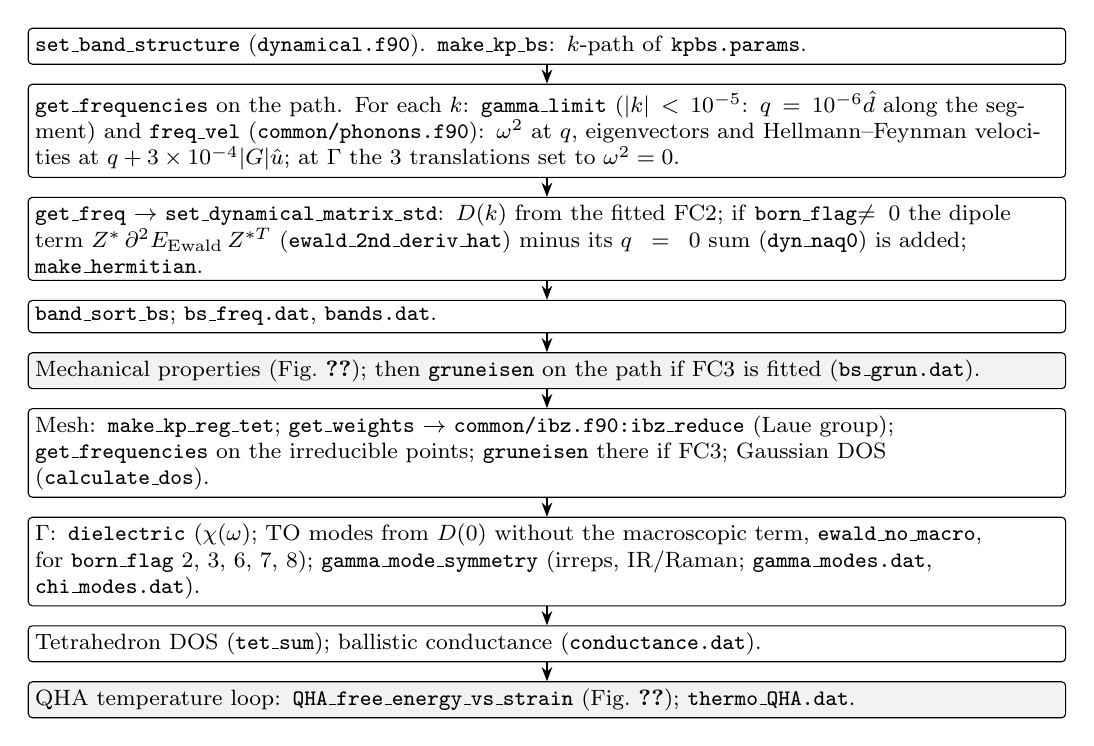
\begin{tikzpicture}[node distance=2.4mm]
\node[box=13cm] (k1) {\code{set\_band\_structure} (\code{dynamical.f90}). \code{make\_kp\_bs}: $k$-path of \code{kpbs.params}.};
\node[box=13cm, below=of k1] (k2) {\code{get\_frequencies} on the path. For each $k$: \code{gamma\_limit} ($|k|<10^{-5}$: $q=10^{-6}\hat d$ along the
  segment) and \code{freq\_vel} (\code{common/phonons.f90}): $\omega^2$ at $q$, eigenvectors and Hellmann--Feynman velocities at
  $q+3\times10^{-4}|G|\hat u$; at $\Gamma$ the 3 translations set to $\omega^2=0$.};
\node[box=13cm, below=of k2] (k3) {\code{get\_freq} $\to$ \code{set\_dynamical\_matrix\_std}: $D(k)$ from the fitted FC2; if \code{born\_flag}$\ne0$
  the dipole term $Z^*\,\partial^2E_{\rm Ewald}\,Z^{*T}$ (\code{ewald\_2nd\_deriv\_hat}) minus its $q=0$ sum (\code{dyn\_naq0}) is added;
  \code{make\_hermitian}.};
\node[box=13cm, below=of k3] (k4) {\code{band\_sort\_bs}; \code{bs\_freq.dat}, \code{bands.dat}.};
\node[box=13cm, below=of k4, fill=gray!10] (k5) {Mechanical properties (Fig.~\ref{fig:mech}); then \code{gruneisen} on the path if FC3 is fitted (\code{bs\_grun.dat}).};
\node[box=13cm, below=of k5] (k6) {Mesh: \code{make\_kp\_reg\_tet}; \code{get\_weights} $\to$ \code{common/ibz.f90:ibz\_reduce} (Laue group);
  \code{get\_frequencies} on the irreducible points; \code{gruneisen} there if FC3; Gaussian DOS (\code{calculate\_dos}).};
\node[box=13cm, below=of k6] (k7) {$\Gamma$: \code{dielectric} ($\chi(\omega)$; TO modes from $D(0)$ without the macroscopic term, \code{ewald\_no\_macro},
  for \code{born\_flag} 2, 3, 6, 7, 8); \code{gamma\_mode\_symmetry} (irreps, IR/Raman; \code{gamma\_modes.dat}, \code{chi\_modes.dat}).};
\node[box=13cm, below=of k7] (k8) {Tetrahedron DOS (\code{tet\_sum}); ballistic conductance (\code{conductance.dat}).};
\node[box=13cm, below=of k8, fill=gray!10] (k9) {QHA temperature loop: \code{QHA\_free\_energy\_vs\_strain} (Fig.~\ref{fig:mech}); \code{thermo\_QHA.dat}.};
\foreach \u/\v in {k1/k2,k2/k3,k3/k4,k4/k5,k5/k6,k6/k7,k7/k8,k8/k9} \draw[arr] (\u) -- (\v);
\end{tikzpicture}
\caption{Lattice dynamics, in the order of \code{dynamical.f90:set\_band\_structure}. Grey: parts shown in Fig.~\ref{fig:mech}.}
\label{fig:ld}
\end{figure}

%==============================================================================
\section{Elastic constants from the Born--Huang brackets (9.2)}\label{sec:elastic}
%==============================================================================
\paragraph{Motivation.} The elastic constants were computed as $\Sym(A)-\Sym(\delta\sigma)$. On the exact
relaxed ZnO model this gave $C_{12}$ 171 instead of 221\,GPa, $C_{13}$ 137 instead of 197, $C_{44}$ 108
instead of 78, $C_{66}$ 146 instead of 121; the diagonal constants were right. All earlier FOCEX elastic
constants, moduli, sound speeds and Debye temperatures were affected. The cause: the step from
$\tfrac12\sum u\Phi u$ to $-\tfrac14\sum(u_i-u_j)\Phi_{ij}(u_i-u_j)$ needs
$\Phi^{\alpha\beta}_{ij}=\Phi^{\beta\alpha}_{ij}$, true for central pair forces only; in general only
$\Phi^{\alpha\beta}_{ij}=\Phi^{\beta\alpha}_{ji}$ holds. The part of each 3$\times$3 block antisymmetric in
its Cartesian indices is lost.

\paragraph{Algorithm.} With the brackets of Eq.~\eqref{eq:bracket} and the reference stress $\sigma$,
\begin{equation}
c_{\alpha\beta\gamma\delta}=\Sym\Big\{[\alpha\gamma,\beta\delta]+[\beta\gamma,\alpha\delta]-[\alpha\beta,\gamma\delta]
+\tfrac12(\delta_{\alpha\beta}\sigma_{\gamma\delta}+\delta_{\gamma\delta}\sigma_{\alpha\beta})
-\delta_{\alpha\gamma}\sigma_{\beta\delta}-\delta_{\beta\delta}\sigma_{\alpha\gamma}\Big\}
-\frac1V\Sym(Q\Gamma Q).
\end{equation}
$\Sym$ is the average over $\alpha\leftrightarrow\beta$, $\gamma\leftrightarrow\delta$ and
$(\alpha\beta)\leftrightarrow(\gamma\delta)$. $Q$ is the first moment of FC2 (sum over $j$ of
$\Phi_{\tau j}$ times the bond vector), the coupling of strain and internal displacements, and $\Gamma$ the
pseudo-inverse of the $q=0$ FC2 matrix between sublattices; the last term is the internal relaxation. The
$(\alpha\beta)\leftrightarrow(\gamma\delta)$ average was added in 9.3: without it the tensor of a
non-hydrostatically stressed state is not pair-symmetric (ZnO model at 15\,GPa: $H_{13}$ 51.452 and
$H_{31}$ 51.420, exact 51.436 = the average).

\paragraph{Implementation.} \code{elastic\_born\_huang} (\code{dynamical.f90}), used by \code{mechanical},
\code{mechanical0} and the relaxation. Results in \code{mech.dat}. The stress is that of
\code{stress.params} (point-group averaged since 9.6). Since 9.7, with Born charges on, the constants from
the short-range FC2 alone go to the log only (with a warning); \code{mech.dat} keeps the long-wave tensor
(Section~\ref{sec:longwave}).

\paragraph{Validation.} \code{REFERENCE/exact\_model/bprime/elastic\_check.py} against the model's strain
Hessian: within $6\times10^{-10}$\,GPa for relaxed ZnO, CaF$_2$ and CaF$_2$ under 14.5\,GPa; 0.2\,GPa on the
stressed ZnO and HfO$_2$ references, whose residual forces are not in the formula. Ge (DFT): $C_{11}$,
$C_{12}$, $C_{44}$ = 121.1, 55.0, 53.9\,GPa; the old code gave $C_{12}$ 68.0 $>$ $C_{44}$ 47.4.

%==============================================================================
\section{\texorpdfstring{$B_0'$ from FC3 and the quasi-harmonic model (9.2)}{B0' from FC3 and the quasi-harmonic model (9.2)}}\label{sec:qha}
%==============================================================================
\paragraph{Motivation.} The old QHA took $V(T)$ as a Boltzmann-weighted average over strains with an
artificial temperature, the expansion coefficient as a secant, $B(T)=B_0(1-\epsilon(4+3\langle\gamma\rangle))$,
and a static energy quadratic in $\Delta V$ (equivalent to $B_0'=-1$).

\paragraph{Algorithm.} \emph{$B_0'$.} Let $\eta_1$, $u_1$ be the strain and internal relaxation per unit
pressure (path $p_1$). Deform the crystal by $\pm\lambda p_1$: FC2 becomes $\Phi\pm\lambda\,\delta\Phi$ with
$\delta\Phi_{\tau j}=\sum_k\Psi_{\tau jk}(S_k-S_\tau)$, $S_j=\eta_1 X_j+u_1(\tau_j)$, the bond vectors and the
pressure change accordingly, and the relaxed bulk modulus $B(\pm\lambda)$ is computed from the elastic
constants of the deformed crystal. Then
\begin{equation}
B_0'=\frac{B(+\lambda)-B(-\lambda)}{2\lambda},\qquad\lambda=10^{-4}\ \mathrm{eV}/\text{\AA}^3.
\end{equation}
FC4 does not enter. Without FC3, $B_0'=1+2\gamma$ with Leont'ev's $\gamma=1.5(3-4x^2)/(1+2x^2)$,
$x=v_t/v_l$ (Dugdale--MacDonald). \emph{QHA.} $F(V,T)=E_{\rm st}(V)+F_{\rm ph}(V,T)$ on 61 isotropic strains
from $-5$\,\% to $+10$\,\%, with $\omega(V)$ from the mode Gr\"uneisen parameters. The static part is
Murnaghan's,
\begin{equation}
P_{\rm st}(V)=P_0+\frac{B_0}{B_0'}\Big[\Big(\frac{V_0}V\Big)^{B_0'}-1\Big],\qquad E_{\rm st}=-\int P_{\rm st}\,dV ,
\end{equation}
with $B_0$ the Reuss modulus and $P_0$ the residual pressure. $P=-\partial F/\partial V$ is summed
analytically; $V(T)$ is the root of $P=0$ (local cubic fit); $B_T=-V\,dP/dV$ there;
$\alpha_V=(\partial P/\partial T)_V/B_T=d\ln V/dT$; the linear coefficient is $\alpha_V/3=d\ln L/dT$;
$C_p=C_v+VTB_T\alpha_V^2$. Harmonic-only fits use Leont'ev's $\gamma$ for all modes plus the term
$P=NkT/V$ ($F=-NkT\ln(V/V_0)$).

\paragraph{Implementation.} Figure~\ref{fig:mech} shows the order of these steps in the code and which of them use the
short-range FC2 only when Born charges are on. \code{pressure\_derivative\_b} and \code{QHA\_free\_energy\_vs\_strain}
(\code{dynamical.f90}); \code{thermo\_QHA.dat} (column 11 $B_T(T)/B_T(T{<}8\,\mathrm K)$ since 9.3, columns 12,
13 $B_T$ and $B_0$). The wrong $B_0'$ of \code{cubic\_elastic} is no longer computed (9.7). With Born charges
the QHA takes $B_0$ and the sound speeds from the long-wave $E=0$ tensor (9.7). The FC2-only rule
$1+2\gamma$ is commit \code{3b638a7}, contained in the tag \code{focex-9.2} (\code{acf1968}).

\paragraph{Validation.} FOCEX on relaxed, cubic-truncated exact-model inputs
(\code{bprime/mkrelaxed.py}): ZnO $B=288.001543$\,GPa, $B'=-0.157427$; CaF$_2$ 587.376258 and 0; equal to
full relaxations under pressure. Evaluating the second-order term with the plain bracket sum instead gives
$B'=-0.064$ for ZnO (wrong, same cause as Section~\ref{sec:elastic}). $\alpha$ equals the numerical
$d\ln L/dT$ of the table to 0.8\,\% (ZnO model with FC3) and 0.7\,\% (FC2 only).

%------------------------------------------------------------------------------
\begin{figure}[tbp]
\centering
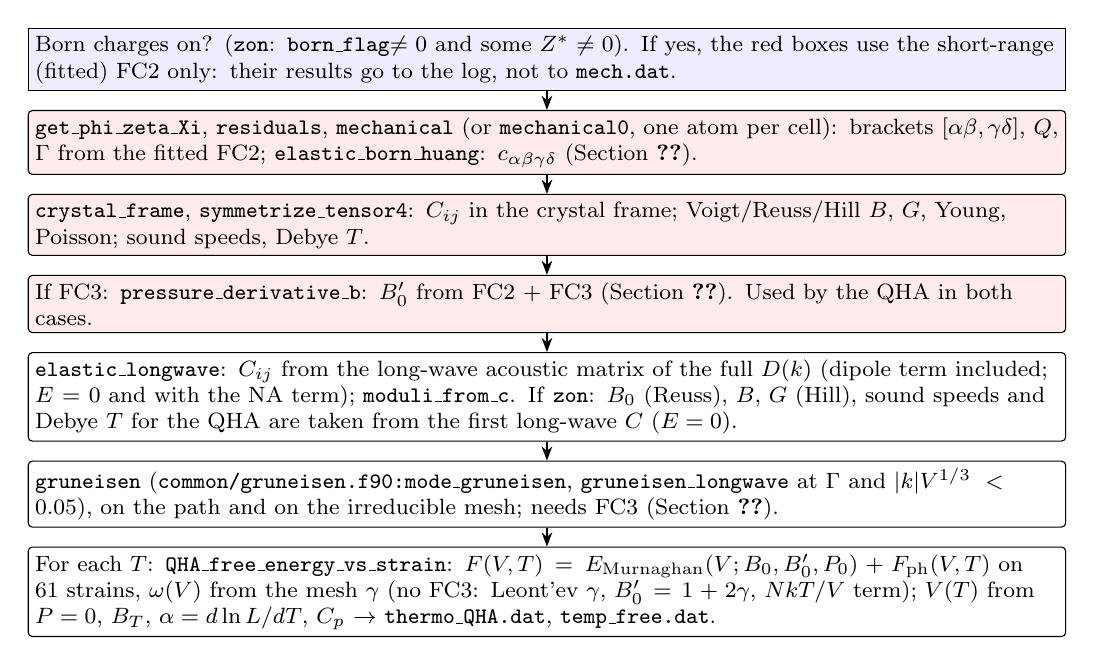
\begin{tikzpicture}[node distance=2.4mm]
\node[dec=13cm] (m0) {Born charges on? (\code{zon}: \code{born\_flag}$\ne0$ and some $Z^*\ne0$). If yes, the red boxes use the
  short-range (fitted) FC2 only: their results go to the log, not to \code{mech.dat}.};
\node[sr=13cm, below=of m0] (m1) {\code{get\_phi\_zeta\_Xi}, \code{residuals}, \code{mechanical} (or \code{mechanical0}, one atom per cell):
  brackets $[\alpha\beta,\gamma\delta]$, $Q$, $\Gamma$ from the fitted FC2; \code{elastic\_born\_huang}: $c_{\alpha\beta\gamma\delta}$ (Section~\ref{sec:elastic}).};
\node[sr=13cm, below=of m1] (m2) {\code{crystal\_frame}, \code{symmetrize\_tensor4}: $C_{ij}$ in the crystal frame; Voigt/Reuss/Hill $B$, $G$, Young, Poisson;
  sound speeds, Debye $T$.};
\node[sr=13cm, below=of m2] (m3) {If FC3: \code{pressure\_derivative\_b}: $B_0'$ from FC2 + FC3 (Section~\ref{sec:qha}). Used by the QHA in both cases.};
\node[box=13cm, below=of m3] (m4) {\code{elastic\_longwave}: $C_{ij}$ from the long-wave acoustic matrix of the full $D(k)$ (dipole term included;
  $E=0$ and with the NA term); \code{moduli\_from\_c}. If \code{zon}: $B_0$ (Reuss), $B$, $G$ (Hill), sound speeds and Debye $T$
  for the QHA are taken from the first long-wave $C$ ($E=0$).};
\node[box=13cm, below=of m4] (m5) {\code{gruneisen} (\code{common/gruneisen.f90:mode\_gruneisen}, \code{gruneisen\_longwave} at $\Gamma$ and
  $|k|V^{1/3}<0.05$), on the path and on the irreducible mesh; needs FC3 (Section~\ref{sec:grun}).};
\node[box=13cm, below=of m5] (m6) {For each $T$: \code{QHA\_free\_energy\_vs\_strain}: $F(V,T)=E_{\rm Murnaghan}(V;B_0,B_0',P_0)+F_{\rm ph}(V,T)$ on
  61 strains, $\omega(V)$ from the mesh $\gamma$ (no FC3: Leont'ev $\gamma$, $B_0'=1+2\gamma$, $NkT/V$ term);
  $V(T)$ from $P=0$, $B_T$, $\alpha=d\ln L/dT$, $C_p$ $\to$ \code{thermo\_QHA.dat}, \code{temp\_free.dat}.};
\foreach \u/\v in {m0/m1,m1/m2,m2/m3,m3/m4,m4/m5,m5/m6} \draw[arr] (\u) -- (\v);
\end{tikzpicture}
\caption{Mechanical properties, Gr\"uneisen parameters and QHA, in the order of \code{dynamical.f90:set\_band\_structure}
(mechanical properties come right after the band structure, before the Gr\"uneisen parameters). Red: short-range FC2 only
when Born charges are on; $B_0'$ is then still from the short-range FCs.}
\label{fig:mech}
\end{figure}

%==============================================================================
\section{Mode Gr\"uneisen parameters (9.2)}\label{sec:grun}
%==============================================================================
\paragraph{Motivation.} FOCEX built the matrix $W$ below with the phase $e^{iq\cdot(R+\tau'-\tau)}$, while
its eigenvectors come from a dynamical matrix with $e^{iq\cdot R}$; $\gamma$ was right only at $q=0$ and off
by up to 3.2 on the exact HfO$_2$ model. THERMACOND's routine had no internal relaxation. At $\Gamma$ the
acoustic $\gamma$ is $0/0$; evaluated at small $q$ it loses digits as $\varepsilon_{\rm mach}/q^2$.

\paragraph{Algorithm.} Under an isotropic strain $\epsilon$ with relaxed internal coordinates the atoms
move by $\epsilon\,y_{R\tau}$, $y_{R\tau}=R+\tau+\xi_\tau$, $\xi_\tau=-\sum_{\tau'}\Gamma_{\tau\tau'}\Tr Q_{\tau'}$. Then
\begin{equation}
\gamma_s(q)=-\frac{\langle e_s|W(q)|e_s\rangle}{6\,\omega_s^2(q)},\qquad
W_{\tau\alpha,\tau'\beta}(q)=\sum_{R'}\sum_k\frac{\Psi^{\alpha\beta\gamma}_{0\tau,R'\tau',k}\,y_k^\gamma}{\sqrt{m_\tau m_{\tau'}}}e^{iq\cdot R'} ,
\end{equation}
with the same phase as the dynamical matrix $D$. Along $\hat q$ write $D=D_0+qD_1+q^2D_2$ and
$W=W_0+qW_1+q^2W_2$. With $T$ the mass-weighted rigid translations, $P=1-TT^\dagger$ and
$G=(PD_0P)^+$,
\begin{equation}
A=T^\dagger D_2T-T^\dagger D_1GD_1T,
\end{equation}
\begin{equation}
B=T^\dagger W_2T-T^\dagger W_1GD_1T-T^\dagger D_1GW_1T+T^\dagger D_1GW_0GD_1T,
\end{equation}
\begin{equation}
\gamma_s(\hat q)=-\frac{b_s}{6a_s},
\end{equation}
with $a_s$, $u_s$ the eigenvalues and eigenvectors of $A$ and $b_s=u_s^\dagger Bu_s$ (within a degenerate
subspace, the eigenvalues of $B$ there). $W_0$, $W_1$, $W_2$ are exact sums over the FC3 terms; $D_0$,
$D_1$, $D_2$ come from the code's own $D$ (NA term included) at $\pm h,\pm2h,\pm3h$, $h=10^{-3}|G|$. The limit
is used for the three translations at $\Gamma$ and for the acoustic modes at $0<|k|V^{1/3}<0.05$. The
eigenvectors at $k$ are those of $D(k)$, with $W$ diagonalized inside each degenerate set (tolerance
$10^{-7}\max\omega^2$).

\paragraph{Implementation.} Module \code{gruneisen\_rules} (\code{common/gruneisen.f90}): \code{mode\_gruneisen},
\code{gruneisen\_longwave}, \code{internal\_strain\_trace}; shared with THERMACOND, each code passing its
FC3 terms (\code{w\_terms\_set}) and its dynamical matrix. Log section \code{GRUNEISEN\_LONGWAVE}.
Derivation: \code{generalized\_huang.tex}, Part III.

\paragraph{Validation.} Exact HfO$_2$ model: the direct values approach the limit as $q^2$ down to
$q\simeq3\times10^{-4}$\,\AA$^{-1}$; at $q=10^{-3}$ for CaF$_2$, ZnO, HfO$_2$, four directions, with and
without relaxation, $\max|\gamma^{\rm direct}-\gamma(\hat q)|\le8\times10^{-6}$. FOCEX on the cubic-truncated
HfO$_2$ model, ranks 1--3: equal to the exact $\gamma$ to the printed $5\times10^{-5}$ at all 519 path points
off $\Gamma$; THERMACOND to its 4 digits; $\Gamma$ limit $-1.691288$, $-1.344395$, $-0.658566$ in both.

%==============================================================================
\section{Standard errors of the fitted FCs, sd(rank) (9.2)}\label{sec:sd}
%==============================================================================
\paragraph{Motivation.} For \code{enforce\_inv}=1 the errors were read from an unset array; for 0 they were
scaled by $\sqrt{c}$ and divided again by $\sqrt N$.

\paragraph{Algorithm.} With the SVD $\bA\bK=\mathbf U\bW\mathbf V^T$ (singular values $w_k$, cut
$w_c=c\,w_{\max}$), the residual variance per row $s^2=\|\bA\bK\by-\bb\|^2/(N-n_K)$ and the filter
$f(w)=w^4/(w^6+w_c^6)$ ($=1/w^2$ well above the cut),
\begin{equation}
\sigma_j=s\,\sqrt{\big[\bK\mathbf Vf(\bW)\mathbf V^T\bK^T\big]_{jj}} .
\end{equation}
For \code{enforce\_inv}=0 the same holds with $\bK=1$ and the stacked matrix. sd(rank) is the mean $\sigma$ of the irreducible FCs of that rank.

\paragraph{Implementation.} \code{svd\_set} (\code{svd\_ridge.f90}) returns $\mathbf V\,\mathrm{diag}(s\sqrt{f(w)})$,
which \code{fit\_kernel\_basis} maps by $\bK$. The log lists every irreducible FC with its $\sigma$
(\code{write\_independent\_fcs}). In 9.9 the array \code{sd} was enlarged from 4 to 8 entries (the writer
fills 8).

\paragraph{Validation.} Exact ZnO model, ranks 1--3, Gaussian force noise $10^{-3}$: estimated
$s=0.9948\times10^{-3}$, $1.0005\times10^{-3}$, $0.9776\times10^{-3}$ (two seeds; \code{enforce\_inv}=1, 0);
rms of $(x-x_{\rm exact})/\sigma$ 1.03 for FC2, 0.84--0.90 for FC3; 72--76\,\% within one $\sigma$. A jackknife
(5 refits leaving out 20 of the 100 snapshots): ratio to the SVD $\sigma$, median 1.04 (FC2), 0.91 (FC3), rms
ratio 0.96. Open: why the FC3 errors are 10--15\,\% below the estimate.

%==============================================================================
\section{Relaxation of an unrelaxed reference (9.3)}\label{sec:relax}
%==============================================================================
\paragraph{Motivation.} A DFT reference may carry residual forces (FC1) and stress. Downstream quantities
(phonons, elastic constants, QHA) should be those of the relaxed structure.

\paragraph{Algorithm.} The static displacement is $S_{R\tau}=\eta\,(R+\tau)+u_{0,\tau}$, with $\eta$ the
strain and $u_0$ the internal shifts ($u_0$ of atom 1 held at 0). The Taylor energy
Eq.~\eqref{eq:taylor} with $u=S$ is minimized over $(\eta,u_0)$. The FCs are re-expanded about the minimum,
\begin{equation}
\Pi'=\Pi+\Phi S+\tfrac12\Psi SS+\tfrac16\chi SSS,\qquad K=\Phi+\Psi S+\tfrac12\chi SS,\qquad \Psi'=\Psi+\chi S,
\end{equation}
with $S_j-S_\tau$ in place of $S_j$ (equal by the sum rules and independent of the image chosen). Stage 1
relaxes $u_0$ in the reference cell. Stage 2 takes Newton steps in the six symmetric strain components,
with $u_0$ relaxed at each point of the path (a force-free path). Along the path
$F(t)=1+t\Delta$ the second Piola--Kirchhoff stress $S$ is integrated by
\begin{equation}
\frac{dS_{ab}}{dt}=J\,F^{-1}_{aj}F^{-1}_{bk}F^{-1}_{cl}F^{-1}_{dm}\,c^{\rm rel}_{jklm}\,\dot E_{cd},
\qquad \dot E=\tfrac12(\Delta^TF+F^T\Delta),\quad J=\det F ,
\end{equation}
with $c^{\rm rel}$ the relaxed elastic tensor of the current state (Section~\ref{sec:elastic}). The rotation
is removed from the accumulated deformation gradient after each step by polar decomposition. The ALATDYN
paper's strain Hessian $A=-\tfrac12\sum K\,d\,d$ is not used: it is the symmetrized form of
Section~\ref{sec:elastic} and is wrong off the Cauchy case.

\paragraph{Implementation.} \code{relax\_reference} (\code{FOCEX/relax\_reference.f90}; flow in Fig.~\ref{fig:relax}), switched on by
\code{default.params} line 5 = 1 (any other value is off). After it, the lattice, positions and grids are
strained by $1+\eta$ and shifted by $u_0$; the re-expanded FCs are projected on the irreducible FCs and used
downstream; \code{stress.params} is then read as 0. The unrelaxed fit is kept as \code{fcN\_unrelaxed.dat},
\code{fcN\_irr\_unrelaxed.dat}, \code{lat\_fc\_unrelaxed.dat}; \code{POSCAR\_relaxed} is written. Since 9.7
the average force per atom is removed from FC1 before relaxing ($\sum_\tau\Pi_\tau=0$), and the fractional
translations of the space group are re-derived for the relaxed cell.

\paragraph{Validation.} Exact ZnO model (stressed 14.9\,GPa, FC1 0.032\,eV/\AA, ranks 1--4,
\code{enforce\_inv}=1) against the model's own minimum: strain $7.8\times10^{-10}$, $u_0$ $1.3\times10^{-9}$\,\AA,
FC2 $2.7\times10^{-6}$\,eV/\AA$^2$, FC3 $5\times10^{-7}$; residual stress $2\times10^{-10}$\,GPa; 3 strain steps.
With ranks 1--3 the strain is off by $10^{-5}$ (FC4 missing). With the paper's $A$ the first version gave ZnO
strain $-0.01831$ against the exact $-0.017837$. Monoclinic HfO$_2$ model (\code{HfO2r}, 12 atoms, no
charges, 4 November): strain $1.3\times10^{-9}$, $u_0$ $2.9\times10^{-9}$\,\AA, FC2 $7.4\times10^{-8}$ (of 6.55),
FC3 $5.1\times10^{-8}$ (of 2.37); stress after $8.7\times10^{-15}$\,GPa.

%------------------------------------------------------------------------------
\begin{figure}[tbp]
\centering
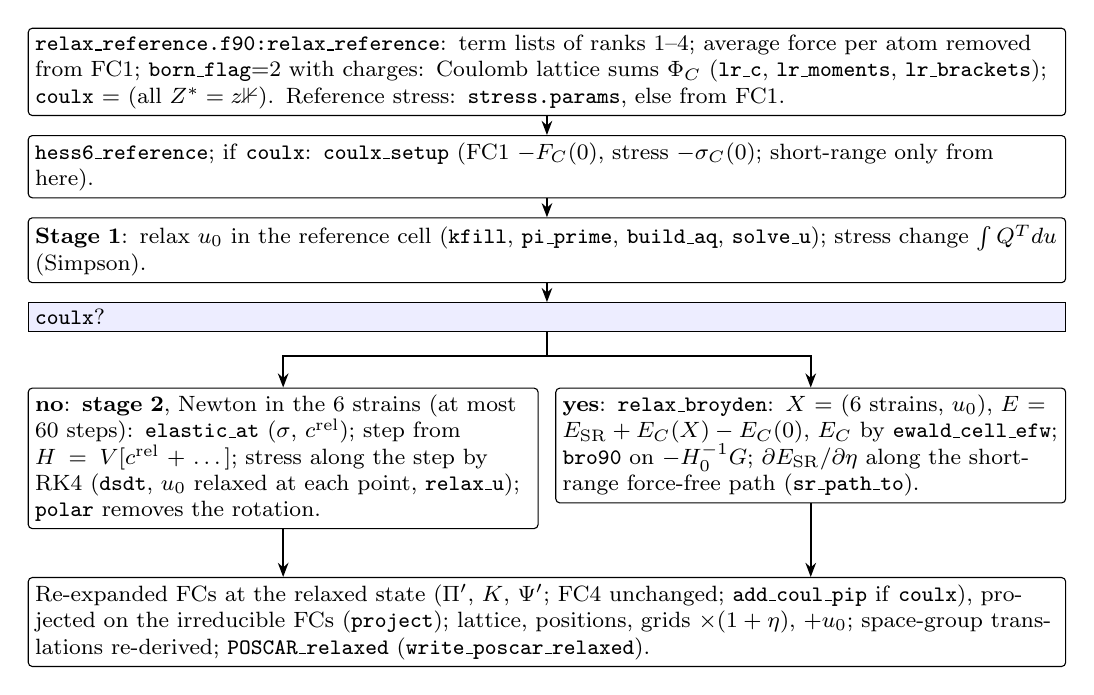
\begin{tikzpicture}[node distance=2.4mm]
\node[box=13cm] (r1) {\code{relax\_reference.f90:relax\_reference}: term lists of ranks 1--4; average force per atom removed from FC1;
  \code{born\_flag}=2 with charges: Coulomb lattice sums $\Phi_C$ (\code{lr\_c}, \code{lr\_moments}, \code{lr\_brackets});
  \code{coulx} = (all $Z^*=z\mathbb 1$). Reference stress: \code{stress.params}, else from FC1.};
\node[box=13cm, below=of r1] (r2) {\code{hess6\_reference}; if \code{coulx}: \code{coulx\_setup} (FC1 $-F_C(0)$, stress $-\sigma_C(0)$; short-range only from here).};
\node[box=13cm, below=of r2] (r3) {\textbf{Stage 1}: relax $u_0$ in the reference cell (\code{kfill}, \code{pi\_prime}, \code{build\_aq}, \code{solve\_u});
  stress change $\int Q^T du$ (Simpson).};
\node[dec=13cm, below=of r3] (r4) {\code{coulx}?};
\node[box=6.3cm, below=7mm of r4.south west, anchor=north west] (r5) {\textbf{no}: \textbf{stage 2}, Newton in the 6 strains
  (at most 60 steps): \code{elastic\_at} ($\sigma$, $c^{\rm rel}$); step from $H=V[c^{\rm rel}+\dots]$; stress along the step
  by RK4 (\code{dsdt}, $u_0$ relaxed at each point, \code{relax\_u}); \code{polar} removes the rotation.};
\node[box=6.3cm, below=7mm of r4.south east, anchor=north east] (r6) {\textbf{yes}: \code{relax\_broyden}: $X$ = (6 strains, $u_0$),
  $E=E_{\rm SR}+E_C(X)-E_C(0)$, $E_C$ by \code{ewald\_cell\_efw}; \code{bro90} on $-H_0^{-1}G$; $\partial E_{\rm SR}/\partial\eta$ along
  the short-range force-free path (\code{sr\_path\_to}).};
\node[fit=(r5)(r6),inner sep=0pt] (rb) {};
\node[box=13cm, anchor=north west] (r7) at ([yshift=-6mm]rb.south -| r1.west) {Re-expanded FCs at the relaxed state ($\Pi'$, $K$, $\Psi'$; FC4 unchanged; \code{add\_coul\_pip} if \code{coulx}),
  projected on the irreducible FCs (\code{project}); lattice, positions, grids $\times(1+\eta)$, $+u_0$; space-group translations
  re-derived; \code{POSCAR\_relaxed} (\code{write\_poscar\_relaxed}).};
\draw[arr] (r1)--(r2); \draw[arr] (r2)--(r3); \draw[arr] (r3)--(r4);
\draw[arr] (r4.south) -- ++(0,-3mm) -| (r5.north); \draw[arr] (r4.south) -- ++(0,-3mm) -| (r6.north);
\draw[arr] (r5) -- (r5 |- r7.north); \draw[arr] (r6) -- (r6 |- r7.north);
\end{tikzpicture}
\caption{Relaxation of the reference (\code{default.params} line 5 = 1; Sections~\ref{sec:relax}, \ref{sec:coulrelax}).}
\label{fig:relax}
\end{figure}

%==============================================================================
\section{\texorpdfstring{IR/Raman activity and irreducible representations at $\Gamma$ (9.4)}{IR/Raman activity and irreducible representations at Gamma (9.4)}}
%==============================================================================
\paragraph{Motivation.} Users need the symmetry labels and the IR/Raman activity of the $\Gamma$ modes. The
character tables are computed rather than looked up, so that the routine also serves other problems
(electrons, little groups).

\paragraph{Algorithm.} At $q=0$ the modes transform under the space group modulo lattice translations.
Operation $g=\{S|\bt\}$ takes atom $k$ to $\mathrm{img}(k,g)$ and acts on a displacement pattern by
$\Gamma(g)_{3(\mathrm{img}-1)+a,\,3(k-1)+b}=S_{ab}$. For a degenerate set with eigenvectors $E$ (of $D$ at
$q=0$, NA term direction-averaged) the characters are $\chi(g)=\Tr(E^\dagger\Gamma(g)E)$, and
\begin{equation}
n_{\rm IR}=\frac1{|G|}\sum_g\chi^*(g)\Tr S_g,\qquad
n_{\rm Raman}=\frac1{|G|}\sum_g\chi^*(g)\,\frac{(\Tr S_g)^2+\Tr S_g^2}2 ,
\end{equation}
the multiplicities of the vector and of the symmetric second-rank tensor representation; parity
$\chi(i)/\dim$. Character tables by the class-multiplication method: with classes $K_i$ of sizes $h_i$ and
$K_iK_j=\sum_kc_{ijk}K_k$, the vectors $w_k=h_k\chi(K_k)/d$ of an irrep of dimension $d$ satisfy
$M_iw=w_iw$, $(M_i)_{jk}=c_{ijk}$. The matrices $D^{-1/2}M_iD^{1/2}$ ($D=\mathrm{diag}(h)$) are normal; a random
real combination of their Hermitian and anti-Hermitian parts is diagonalized; $\chi_k=dw_k/h_k$ with
$d^2=|G|/\sum_k|w_k|^2/h_k$.

\paragraph{Implementation.} \code{gamma\_mode\_symmetry} (\code{dynamical.f90}) writes
\code{gamma\_modes.dat}; module \code{point\_group\_rules} (\code{common/point\_group.f90}): \code{pg\_setup},
\code{pg\_reduce}, \code{pg\_write\_table}, \code{pg\_chi\_vector}, \code{pg\_chi\_sym2}. Labels: A/B, E, T,
g/u, $'$/$''$, a serial number only when needed; classes in a fixed order so that the labels do not depend
on the order of the operations. One symmetry tolerance \code{tol\_sym}$=10^{-3}$\,\AA{} (\code{common/params.f90})
for accepting operations and finding atom images. Acoustic modes by their translation weight.

\paragraph{Validation.} \code{REFERENCE/point\_groups/test\_point\_groups.f90}: all 32 point groups (order,
classes, dimensions, orthogonality); $O_h$ $T_{1u}$ = 3 1 0 $-$3 $-$1 $-$1 $-$1 0 1 1 as the standard table.
\code{gamma\_modes.dat}: ZnO $2A_1+2B_2+2E_2+2E_1$; HfO$_2$ $9A_g+9A_u+9B_g+9B_u$ (acoustic $A_u+2B_u$); LaP
$2T_{1u}$. LaP IR strength 0.962 = 3$\times$0.3207 of the dielectric table.

%==============================================================================
\section{\texorpdfstring{Reading some ranks and fitting the others, \code{include\_fc}=2 (9.5)}{Reading some ranks and fitting the others, include\_fc=2 (9.5)}}\label{sec:incl2}
%==============================================================================
\paragraph{Motivation.} One may want to keep FC2 from a dense harmonic data set and fit only FC3, or rerun a
part of the analysis without refitting everything.

\paragraph{Algorithm.} Partition $\bx=(\bx_{\rm fit},\bx_{\rm read})$. Force rows and invariance rows
become
\begin{equation}
\bA_{\rm fit}\bx_{\rm fit}=\bb-\bA_{\rm read}\bx_{\rm read},\qquad
\bC_{\rm fit}\bx_{\rm fit}=\bd-\bC_{\rm read}\bx_{\rm read} .
\end{equation}
The Huang rows contain FC2 only and are dropped when FC2 is read. The irreducible values of a read group
$g$ are the least-squares solution of $\sum_tM_{t,t'}x_{t'}=f_t$ over its terms $t$ (absent terms
$f_t=0$); the residual is logged.

\paragraph{Implementation.} \code{include\_fc} is \code{structure.params} line 4. \code{read\_fcs}
(\code{ios.f90}) reads \code{fcN.dat} and the earlier \code{lat\_fc.dat}, and matches atoms by (sublattice,
cell), whatever the numbering. Module \code{given\_fcs} (\code{xfull}, \code{full\_col}); force-row
right-hand side in \code{setup\_amatrix.f90}; invariance right-hand side and \code{merge\_given\_fcs} in
\code{invariance\_ranks.f90}. After the fit the read ranks count as fitted, so all output is that of a full
fit. \code{fcN.dat} and \code{fcN\_irr.dat} carry 8 significant digits (format \code{g15.8}) since 3 November
2026. In 9.8: if every included rank is read, the force data, invariance rows and fit are skipped
(relax-only rerun, Section~\ref{sec:coulrelax}).

\paragraph{Validation.} Cubic-truncated HfO$_2$ model: full fits byte-identical; reading FC3, or FC1+FC2,
gives the rest to the printed digits; reading FC2 gives FC3 to $10^{-4}$. Reading FC2 at 7, 8 and 15 digits
gives FC3 relative errors $1.1\times10^{-4}$, $5.3\times10^{-5}$, $2.4\times10^{-9}$: the error is the rounding of
the input. A random relabelling of atoms 13..6500 in \code{lat\_fc.dat} and \code{fcN.dat} gives
byte-identical outputs.

%==============================================================================
\section{\texorpdfstring{\code{born\_flag}=2: hybrid Coulomb subtraction with Coulomb right-hand sides (9.5)}{born\_flag=2: hybrid Coulomb subtraction with Coulomb right-hand sides (9.5)}}\label{sec:hybrid}
%==============================================================================
\paragraph{Motivation.} With \code{born\_flag}=2 FOCEX subtracts a long-range Coulomb force from the DFT
forces, fits the short-range remainder, and adds the dipole term back to the dynamical matrix. With
anisotropic $Z^*$ the harmonic part of the subtracted force was not the term added back (per Zn--O pair
$xz$ 0.170 and $zx$ 0.188 against 0.179). The invariance rows on the short-range part used the total
residual forces and stress, while the dipole FCs alone carry their own (ZnO: deviatoric stress
$(-0.108,-0.108,+0.216)$\,GPa).

\paragraph{Algorithm.} The subtracted force is
\begin{equation}
F_{\rm sub}=F_m(x)-F_m(x_0)-(\Phi_C-\Phi_m)\,u ,
\end{equation}
with $F_m$ the Ewald force of the pair model with couplings $c_{ij}=\Tr(Z_iZ_j^T)/3$ in the dielectric
$\epsilon$; $\Phi_C$ the Coulomb dipole FCs ($e^2Z_tT(R+x_u-x_t)Z_u^T$, $T=-\nabla\nabla\phi_\epsilon$,
$E=0$), equal to the term added back to $D$; and $\Phi_m$ the harmonic part of the pair model. The
harmonic part subtracted is then exactly $\Phi_C$. The fit sees $\bx_{\rm fit}=\bx-\bx_{\rm sub}$, so every
included invariance row gets the right-hand side $-\bC\bx_{\rm sub}$: Huang rows
$-(S_C(\alpha\beta,\gamma\delta)-S_C(\gamma\delta,\alpha\beta))$; rank-2 rotational rows
$-\sum_{a\mu}M(i_1;\alpha_1,a,\mu)\varepsilon_{a\mu\nu}$ with $M=\sum_j\Phi_C(i_1\alpha_1,ja)(X_j-X_{i_1})_\mu$;
rank-3 rotational rows from the FC3 of the pair model. The lattice sums are conditionally convergent;
they come from the small-$q$ expansion of the $E=0$ Ewald sum (central differences with Richardson
extrapolation).

\paragraph{Implementation.} \code{hybrid\_harmonic}, \code{subtract\_coulomb\_force} (\code{ewald\_born.f90});
module \code{coulomb\_lr} (\code{coulomb\_lr.f90}: \code{lr\_brackets}, \code{lr\_moments},
\code{lr\_rot3\_pair}, \code{lr\_rot3\_onsite}); Huang right-hand side in \code{setup\_amatrix.f90},
rotational in \code{invariance\_ranks.f90}. The \code{mech.dat} Huang and rotational checks include the
same terms. No switch: the right-hand sides are always applied when the rows are included. In 9.6 the
correction $\Phi_C-\Phi_m$ is computed for each supercell (it was computed for the first only; GaN with two
supercells gave fits of 2.98, 3.24, 712, 4.95\,\% on identical runs; after the fix 1.719\,\%).
\code{born\_flag}$>2$ prints a warning (9.2): use 0 or 2.

\paragraph{Validation.} Exact SR model plus point charges in $\epsilon=5$ (\code{coulomb/mkcoulomb.py}):
ZnO ranks 1--4 exact to the printed digits, fit 0.000\,\%. Cubic HfO$_2$ ranks 1--3: fit 0.000\,\% with the
right-hand sides; 0.095\,\% without the Huang part, 0.510\,\% without the rotational part, 0.523\,\% without
both. User's ZnO (DFT, \code{born\_flag}=2): fit 1.720\,\%$\to$1.269\,\% (hybrid)$\to$1.232\,\% (rank-3 rotational
right-hand side).

%==============================================================================
\section{Elastic constants from the long-wave sound speeds (9.5)}\label{sec:longwave}
%==============================================================================
\paragraph{Motivation.} The bracket route of Section~\ref{sec:elastic} uses the fitted (short-range) FC2
only; with \code{born\_flag}=2 it misses the Coulomb part (user's ZnO: $C_{33}=-58$, $C_{44}=-33$\,GPa). The
long-wave limit of the full dynamical matrix contains it.

\paragraph{Algorithm.} Along 13 directions $\hat q$ (axes, face and body diagonals) the acoustic matrix
$A(\hat q)$ ($\omega^2=q^2\,\mathrm{eig}A$, optical modes folded out exactly as in Section~\ref{sec:grun})
gives, with $\rho$ the mass density,
\begin{equation}
\rho A_{ik}=\sum_{jl}B_{(ik),(jl)}\hat q_j\hat q_l=(C_{ijkl}+\delta_{ik}s_{jl})\hat q_j\hat q_l .
\end{equation}
The 36 brackets $B$ are fitted by least squares (78 equations, rank 36). The stressed Huang relation
$B_{ab,cd}-B_{cd,ab}=\delta_{ab}s_{cd}-\delta_{cd}s_{ab}$ gives the deviatoric stress (15 equations, 5
unknowns; the pressure is invisible to long waves); $C$ follows from $B-\delta_{ik}s_{jl}$, with the
pressure taken from FOCEX's residual stress. With Born charges two tensors are given: $E=0$ (the
macroscopic-field part of the $G=0$ term left out, switch \code{ewald\_no\_macro} in \code{common/ewald.f90})
and with the NA term.

\paragraph{Implementation.} \code{elastic\_longwave} (\code{dynamical.f90}), \code{acoustic\_tensor}
(\code{common/gruneisen.f90}); \code{mech.dat} section \code{ELASTIC\_LONGWAVE}; isotropic moduli of every
tensor by \code{moduli\_from\_c} (table \code{ELASTIC\_MODULI}). For one atom per cell the optical terms are
skipped (they divided by zero).

\paragraph{Validation.} \code{REFERENCE/exact\_model/longwave}: deviatoric stress to $10^{-13}$\,GPa and $C$ to
$5\times10^{-10}$\,GPa (ZnO, HfO$_2$ stressed, CaF$_2$); FOCEX on the relaxed ZnO model equals the strain
Hessian to $10^{-3}$\,GPa. User's ZnO without charges: equal to the bracket route within 0.06\,GPa. Argon:
3.074, 1.540, 1.537\,GPa by both routes.

%==============================================================================
\section{Irreducible wedge from the Laue group (9.5)}
%==============================================================================
\paragraph{Motivation.} FOCEX reduced $k$-meshes with the point group of the lattice. For a crystal of
lower symmetry than its lattice this makes inequivalent points equivalent: CdI$_2$ on an 8$\times$8$\times$8 mesh
had 50 instead of 65 irreducible points.

\paragraph{Algorithm.} The operations are the rotations of the space-group operations (screw axes and
glide planes included) and their products with inversion (time reversal, $\omega(-k)=\omega(k)$). Each
unassigned mesh point starts a star; every member is mapped onto its mesh point modulo $G$; the weight is
the number of mesh points in the star. The representative is the member, folded into the Wigner--Seitz
cell, with the largest $\hat u\cdot k$ for the fixed generic direction $\hat u=(0.9,\sqrt2-1,\sqrt5-2)$:
$\{k:\hat u\cdot k\ge\hat u\cdot Rk\ \forall R\}$ is a fundamental domain, so the irreducible points fill one
wedge.

\paragraph{Implementation.} Module \code{ibz\_rules} (\code{common/ibz.f90}): \code{laue\_operations},
\code{ibz\_reduce}, shared with THERMACOND (whose algorithm it is); the \code{get\_weights} routines of both
codes are wrappers. The ballistic conductance per \AA$^2$ (\code{conductance.dat}) uses mesh values
reconstructed from the wedge through the Laue operations.

\paragraph{Validation.} Against spglib \code{get\_ir\_reciprocal\_mesh} (time reversal) for 9 structures
$\times$ 4 meshes: same stars, weights and wedge. FOCEX regression (Ge, BZO, MoTe$_2$, GeSe): thermodynamic
outputs within 1 in the last printed digit; THERMACOND Ge byte-identical; CdI$_2$ end to end in both codes
equal to spglib.

%==============================================================================
\section{Symmetrized positions, Born charges, dielectric tensor and stress (9.6)}\label{sec:sym96}
%==============================================================================
\paragraph{Motivation.} DFT positions of GaN and ZnO were off the space group by $3$--$8\times10^{-5}$\,\AA,
below \code{tol\_sym}. The operations were found and the FCs symmetrized exactly, but the Huang and
rotational rows use the actual positions: rows that vanish by symmetry got coefficients $10^{-3}$ of the
largest and acted as spurious constraints. GaN: $C_{66}=-7288$\,GPa; ZnO (\code{enforce\_inv}=1): fit 58.7\,\%.

\paragraph{Algorithm.} Repeat until the positions change by less than $10^{-13}$\,\AA{} (at most 50 passes):
\begin{equation}
\bt_g\leftarrow\bt_g-\big\langle R_gX_k+\bt_g-L_{gk}-X_{\mathrm{img}(k,g)}\big\rangle_k,\qquad
X_j\leftarrow\frac1{|G|}\sum_g\big(R_gX_k+\bt_g-L_{gk}\big),\ \mathrm{img}(k,g)=j ,
\end{equation}
with $L_{gk}$ the lattice vector that brings the image back; the centroid is kept. Tensors:
$Z(k)\leftarrow|G|^{-1}\sum_gR_g^TZ(\mathrm{img}(k,g))R_g$, $\epsilon\leftarrow|G|^{-1}\sum_gR_g\epsilon R_g^T$, and the
same for the stress.

\paragraph{Implementation.} \code{symmetrize\_positions} and \code{pointgroup\_average2}
(\code{force\_constant\_symmetries.f90}), called from \code{focex.f90}; \code{symmetry\_init} is rerun. The
symmetric positions enter the rotational rows, the Huang rows and the relaxation; displacements stay
FORCEDISP minus POSCAR, forces as read.

\paragraph{Validation.} GaN: $C_{66}$ $-7288\to110$\,GPa, no imaginary modes. ZnO: 58.7\,\%$\to$1.30\,\%;
\code{enforce\_inv} 0, 1, 2 agree within 4\,GPa. Exact monoclinic HfO$_2$ with positions perturbed by
$5\times10^{-5}$\,\AA: 9.5 fits 92.5\,\% and 1429\,\%, 9.6 0.000\,\% (FC2 $1.7\times10^{-6}$ relative). Exact ZnO
plus Coulomb: tensor change $4\times10^{-16}$, FCs equal to $10^{-9}$ relative.

%==============================================================================
\section{\texorpdfstring{OpenMP and \code{-O3} with unchanged results (9.7)}{OpenMP and -O3 with unchanged results (9.7)}}
%==============================================================================
\paragraph{Motivation.} The relaxation of the monoclinic HfO$_2$ model took 7843\,s, dominated by the SVDs.

\paragraph{Algorithm.} Rule: an OpenMP loop must give the numbers of the serial code. Every parallel loop is
over independent outputs, each computed by one iteration with its sums in the old order. In \code{svdcmp}
the right Householder step is done by column blocks with OpenMP over columns. One SVD gives both the kernel
and the particular solution (\code{kernel\_and\_particular}; there were two SVDs of the same matrix). Batching
the QR rotations was tried and was slower.

\paragraph{Implementation.} \code{svd\_ridge.f90}; threads from \code{common/omp\_threads.f90}:
\code{FOCEX\_NUM\_THREADS} if set; 1 under an MPI launcher; \code{SLURM\_CPUS\_PER\_TASK}; else cores minus
$\max(1,\text{cores}/5)$. Printed in the log and \code{times.dat}. Default build \code{-O3 -fopenmp}
(\code{make DEBUG=1}: \code{-O2 -fcheck=all -fbacktrace}). The U and V dumps are written only with verbose
(2.1\,GB and 572\,MB for HfO$_2$).

\paragraph{Validation.} \code{svdcmp}: bit-identical on a scratch driver (3000$\times$1200, 6000$\times$2400) and on all
HfO$_2$ outputs (\code{cmp}). \code{-O3} against \code{-O2 -fcheck=all}: FCs, frequencies, thermodynamics identical
(4 regression cases, HfO$_2$). HfO$_2$ relaxation 7843\,s $\to$ 6520\,s (\code{-O3}) $\to$ 1596\,s (8 threads). Left
serial: rotational rows (735\,s), translational rows (247\,s), force rows.

%==============================================================================
\section{Coulomb terms in the relaxation; exact Coulomb by Broyden; relax-only reruns (9.7, 9.8)}\label{sec:coulrelax}
%==============================================================================
\paragraph{Motivation.} With \code{born\_flag}=2 the fitted FCs are short-range only; the relaxation of 9.3
had no Coulomb term. In 9.7 the Coulomb FCs entered to second order (lattice sums of $\Phi_C$ at $q=0$,
$E=0$). A second-order Coulomb energy is not rotationally invariant; on the exact HfO$_2$ model with point
charges the strain was off by $1.4\times10^{-4}$ and $u_0$ by $6.4\times10^{-3}$\,\AA.

\paragraph{Algorithm (9.8).} For $Z^*=z\,\mathbb 1$,
\begin{equation}
E(X)=E_{\rm SR}(X)+E_C(X)-E_C(0),\qquad X=(\eta_1..\eta_6,\ u_0\text{ of atoms }2..),
\end{equation}
with $E_C$ the Ewald energy of the pair model ($c_{ij}=\Tr(Z_iZ_j^T)/3$, $\epsilon$ fixed) at the deformed
cell and positions, and $E_{\rm SR}$ the Taylor series of the fitted FCs with FC1 $-F_C(0)$ and
$\sigma_0-\sigma_C(0)$. That split is required: with the total FC1 and stress the short-range part is not
rotationally invariant. $G(X)=\partial E/\partial X=0$ is solved by modified Broyden mixing on
$f=-H_0^{-1}G$, $H_0$ the Hessian at the reference with $\Phi_C$. $\partial E_{\rm SR}/\partial u_0=\Pi'$.
$\partial E_{\rm SR}/\partial\eta$: the stress formula holds only at force-free states, so the short-range
stress is integrated along the short-range force-free path $u_0^*(\eta)$ (Section~\ref{sec:relax}), giving
$V\sigma F^{-T}$, and then carried from $u_0^*$ to $u_0$ at fixed $\eta$ by $\int Q^Tdu$ (Simpson, exact since
$Q$ is quadratic). For anisotropic $Z^*$ the second-order route is kept, with a warning.

\paragraph{Implementation.} \code{relax\_broyden}, \code{coulx\_setup}, \code{gradfun}, \code{sr\_path\_to},
\code{coul\_energy} in \code{relax\_reference.f90}; \code{ewald\_cell\_efw} (\code{ewald\_cell.f90}: energy,
forces, analytic $dE/d\eta$); \code{bro90} (\code{broyden.f90}, copied from SCOP8). The log checks the Ewald
derivative against 4-point differences ($9\times10^{-10}$) and its independence of the Ewald parameter
($2\times10^{-13}$). Relax-only rerun: set \code{include\_fc}=2 for every rank and copy
\code{fcN\_unrelaxed.dat}$\to$\code{fcN.dat}, \code{lat\_fc\_unrelaxed.dat}$\to$\code{lat\_fc.dat}.

\paragraph{Validation.} Exact HfO$_2$ model with point charges (\code{compare\_relaxed.py}): strain
$2.7\times10^{-9}$, $u_0$ $6.5\times10^{-9}$\,\AA, FC2 $1.1\times10^{-7}$, FC3 $9.4\times10^{-8}$ (second-order route:
$1.4\times10^{-4}$, $6.4\times10^{-3}$, $5.8\times10^{-3}$, $1.6\times10^{-2}$); 14 Broyden steps. Relax-only rerun 219\,s
instead of 33\,min, strain equal to the full run to $10^{-7}$. Regression Ge, BZO, MoTe$_2$, GeSe
byte-identical to 9.7.

%==============================================================================
\section{\texorpdfstring{Constrained LASSO with exact invariances (\code{enforce\_inv}=2, 3)}{Constrained LASSO with exact invariances (enforce\_inv=2, 3)}}\label{sec:lasso}
%==============================================================================
\paragraph{Motivation.} The former LASSO penalized the kernel coefficients $\by$; the columns of $\bK$ are
dense mixtures, so sparse FCs are dense in $\by$. On an exact pair model it gave 98/80/376 non-zero
FC2/FC3/FC4 for 11/20/43 true ones, and FC4 wrong.

\paragraph{Algorithm.} With $w_j$ the rms of column $j$ of $\bA$ (floored at $10^{-8}\max w$),
\begin{equation}
\min_\bx\ \frac1{2N}\|\bA\bx-\bb\|^2+\lambda\sum_jw_j|x_j|\quad\text{subject to}\quad\bx=\bx_0+\bK\by .
\label{eq:classo}
\end{equation}
Let $\bz=\bW\bx$ and $\bQ$ an orthonormal basis of the range of $\bW\bK$, $\bz=\bz_0+\bQ\bt$. Then
\begin{equation}
\min_\bt\ \tfrac12\bt^T\bG\bt-\bc^T\bt+\lambda\|\bz_0+\bQ\bt\|_1,\qquad
\bG=\tilde\bA^T\tilde\bA,\ \bc=\tilde\bA^T\bb/\sqrt N,\ \tilde\bA=\bA\bW^{-1}\bQ/\sqrt N .
\end{equation}
For $\lambda\ge\lambda_{\max}=\|\bQ\bc\|_\infty$ (and $\bz_0=0$) the solution is $\bt=0$. The problem is solved as a
quadratic program by a primal--dual interior-point method (Mehrotra predictor--corrector): the Newton step
reduces to $(\bG+\bQ^T\mathbf D\bQ)\delta\bt=\mathrm{rhs}$ with $D_i=4A_iB_i/(A_i+B_i)$, positive definite,
solved by Cholesky. Here $\bx_0=\bx_p$, and $\bK$ is restricted to the directions $\bK_r$ the data resolve
(Section~\ref{sec:filter}). The support is $S=\{j:|z_j|>10^{-8}\max|z|\}$. The \emph{refit} on a support $S$ is the
least-squares problem with the same quadratic terms but without the $L_1$ term, over the FCs in $S$ only
($x_j=0$ exactly for $j\notin S$) and with the invariances still exact: $\bt$ in the null space of $\bQ_{S^c,:}$
(Householder QR with column pivoting). For every $\lambda$ of the grid the code computes both the LASSO solution and
its refit. $\lambda$ is chosen by 5-fold cross-validation on interleaved rows over 40 log-spaced values from
$\lambda_{\max}$ to $10^{-4}\lambda_{\max}$, by the smallest mean held-out error of the model that is returned: the
refit for \code{enforce\_inv}=3, the LASSO solution for 2. Ties within $10^{-13}\langle b^2\rangle$ take the largest
$\lambda$. While the minimum is at the end the grid is extended by two decades, down to $10^{-8}\lambda_{\max}$.

\paragraph{How to read Figs.~\ref{fig:lassoouter} and~\ref{fig:lassoinner}.} Figure~\ref{fig:lassoouter} is the outer
level: the resolved kernel, the variables $\bt$, the quadratic penalties (SVD filter, optional $L_2$ term), the $\lambda$
grid, the cross-validation, the choice of $\lambda^*$ and the final answer. Figure~\ref{fig:lassoinner} is what happens at
one $\lambda$: the LASSO solution, its support $S(\lambda)$, and the refit on $S(\lambda)$. \code{enforce\_inv}=2 and 3 run
exactly the same computation; they differ only in which of the two solutions is used, to score $\lambda$ in the
cross-validation and as the answer (red boxes). With \code{enforce\_inv}=2 the kept FCs are shrunk towards 0 by the
$L_1$ term; with 3 they are the unbiased least-squares values on the selected set.

\paragraph{Implementation.} Module \code{lasso\_constrained} (\code{lasso\_constrained.f90}): \code{classo\_setup},
\code{ipm\_classo}, \code{refit\_support}, \code{classo\_path}, \code{classo\_cv\_res}, \code{classo\_cv},
\code{resolved\_kernel}, \code{null\_space\_qr}; called from \code{lasso\_kernel\_basis}
(\code{constrained\_fit.f90}). \code{FOCEX\_LASSO=old} selects the old method. Table in \code{lasso.dat}. Added
in commit \code{c9edf0a} (27 October 2026). Background and earlier tests:
\code{FOCEX/notes/constrained\_lasso.tex} (24 October; its hard cut and tie tolerance $10^{-10}$ were
replaced later).

\paragraph{Validation.} Exact model (\code{REFERENCE/exact\_model/README.md}): \code{enforce\_inv}=3 selected
exactly the true support (CaF$_2$ 18/61/190, ZnO 2/47/229/553) and the FCs to the written digits;
\code{enforce\_inv}=2 lost no true FC, with FC4 shrinkage $\le3.6\times10^{-4}$ relative. The old grid floor
$10^{-4}\lambda_{\max}$ had lost 76 true FCs on ZnO. Cubic HfO$_2$, ranks 1--3, 1566 unknowns: 24\,min, no true FC
lost, FC1--3 errors 0, $7\times10^{-13}$, $4.5\times10^{-11}$ relative. Interior point against cvxpy/Clarabel: objective
to $10^{-11}$.

\paragraph{LASSO against \code{enforce\_inv}=1 on DFT data (MgO, 9.9 build).} Same data and setup as the MgO run
of Section~\ref{sec:noisecheck}. \code{enforce\_inv}=3 kept 74 of 556 FCs, fit 4.26\,\% (default line 2: 75 kept,
5.69\,\%), interior point \code{info}=2 (not converged at some $\lambda$); \code{enforce\_inv}=1: fit 0.17\,\%. The
phonons are the same ($T_{1u}$ 534.9, maximum 748.9\,cm$^{-1}$, none unstable); Gr\"uneisen median 1.59
(\code{enforce\_inv}=3) against 1.73 (1). Here LASSO removed FCs the data support; the improvement over the
earlier MgO runs came from the SVD cut (Sections~\ref{sec:gap}, \ref{sec:noisecheck}), not from LASSO.

%------------------------------------------------------------------------------
\begin{figure}[p]
\centering
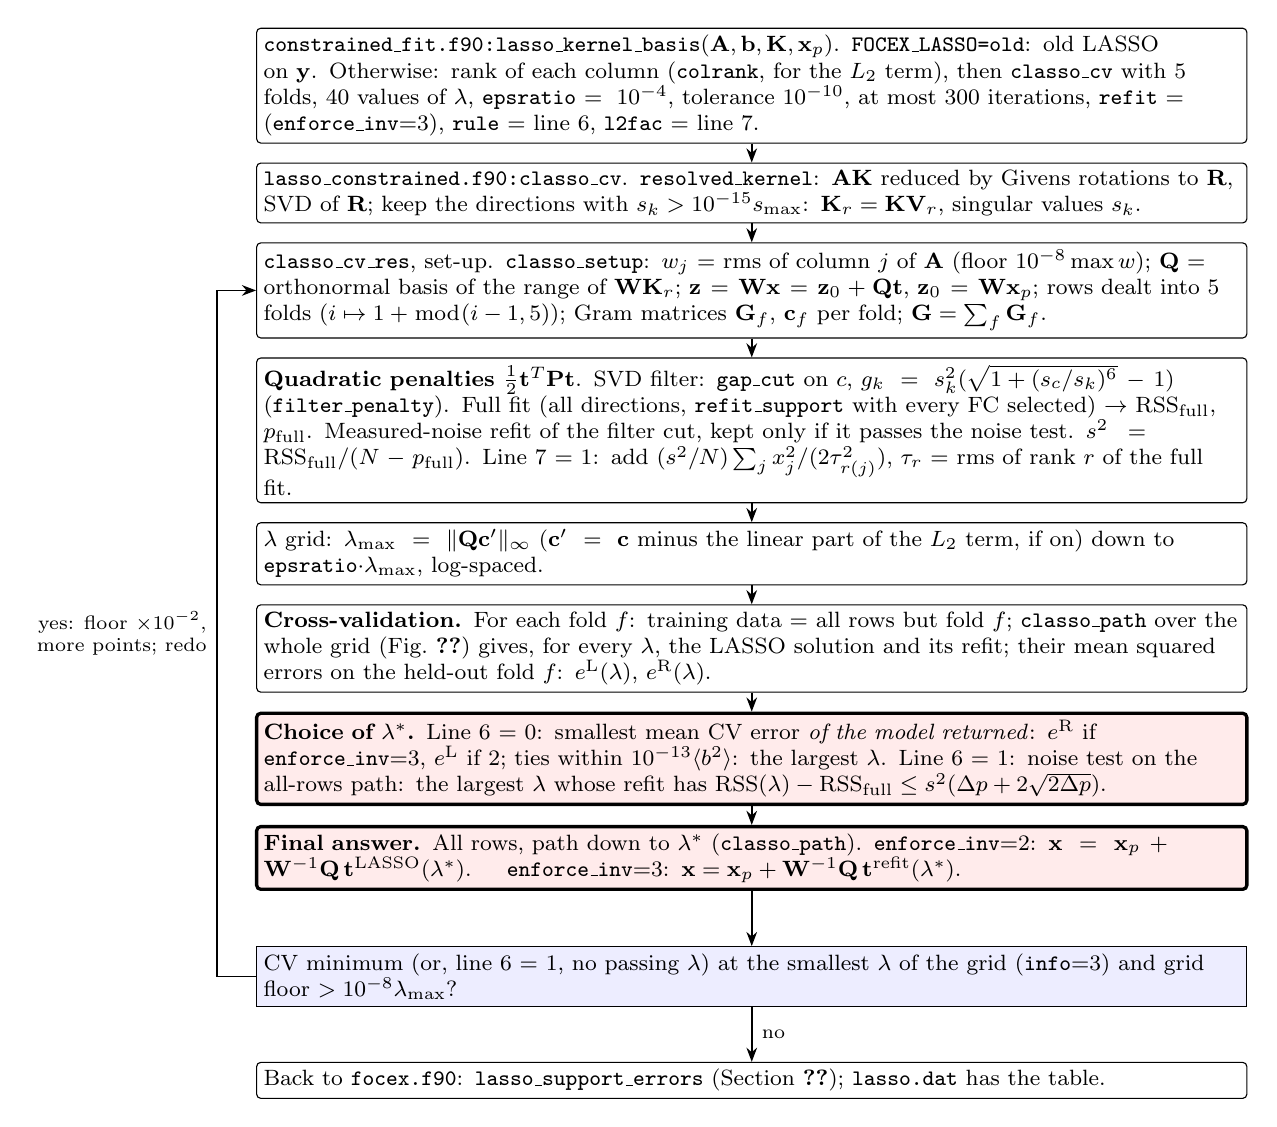
\begin{tikzpicture}[node distance=2.4mm]
\node[box=12.4cm] (g1) {\code{constrained\_fit.f90:lasso\_kernel\_basis}($\bA,\bb,\bK,\bx_p$). \code{FOCEX\_LASSO=old}: old LASSO on $\by$.
  Otherwise: rank of each column (\code{colrank}, for the $L_2$ term), then \code{classo\_cv} with 5 folds, 40 values of
  $\lambda$, \code{epsratio} $=10^{-4}$, tolerance $10^{-10}$, at most 300 iterations, \code{refit} = (\code{enforce\_inv}=3),
  \code{rule} = line 6, \code{l2fac} = line 7.};
\node[box=12.4cm, below=of g1] (g2) {\code{lasso\_constrained.f90:classo\_cv}. \code{resolved\_kernel}: $\bA\bK$ reduced by Givens rotations
  to $\mathbf R$, SVD of $\mathbf R$; keep the directions with $s_k>10^{-15}s_{\max}$: $\bK_r=\bK\mathbf V_r$, singular values $s_k$.};
\node[box=12.4cm, below=of g2] (g3) {\code{classo\_cv\_res}, set-up. \code{classo\_setup}: $w_j$ = rms of column $j$ of $\bA$ (floor $10^{-8}\max w$);
  $\bQ$ = orthonormal basis of the range of $\bW\bK_r$; $\bz=\bW\bx=\bz_0+\bQ\bt$, $\bz_0=\bW\bx_p$; rows dealt
  into 5 folds ($i\mapsto1+\bmod(i-1,5)$); Gram matrices $\bG_f$, $\bc_f$ per fold; $\bG=\sum_f\bG_f$.};
\node[box=12.4cm, below=of g3] (g4) {\textbf{Quadratic penalties} $\tfrac12\bt^T\mathbf P\bt$. SVD filter: \code{gap\_cut} on $c$, $g_k=s_k^2(\sqrt{1+(s_c/s_k)^6}-1)$
  (\code{filter\_penalty}). Full fit (all directions, \code{refit\_support} with every FC selected) $\to$
  $\mathrm{RSS}_{\rm full}$, $p_{\rm full}$. Measured-noise refit of the filter cut, kept only if it passes the noise test.
  $s^2=\mathrm{RSS}_{\rm full}/(N-p_{\rm full})$. Line 7 = 1: add $(s^2/N)\sum_jx_j^2/(2\tau_{r(j)}^2)$, $\tau_r$ = rms of rank $r$ of the full fit.};
\node[box=12.4cm, below=of g4] (g5) {$\lambda$ grid: $\lambda_{\max}=\|\bQ\bc'\|_\infty$ ($\bc'=\bc$ minus the linear part of the $L_2$ term, if on) down to \code{epsratio}$\cdot\lambda_{\max}$, log-spaced.};
\node[box=12.4cm, below=of g5] (g6) {\textbf{Cross-validation.} For each fold $f$: training data = all rows but fold $f$;
  \code{classo\_path} over the whole grid (Fig.~\ref{fig:lassoinner}) gives, for every $\lambda$, the LASSO solution and its refit;
  their mean squared errors on the held-out fold $f$: $e^{\rm L}(\lambda)$, $e^{\rm R}(\lambda)$.};
\node[hl=12.4cm, below=of g6] (g7) {\textbf{Choice of $\lambda^*$.} Line 6 = 0: smallest mean CV error \emph{of the model returned}:
  $e^{\rm R}$ if \code{enforce\_inv}=3, $e^{\rm L}$ if 2; ties within $10^{-13}\langle b^2\rangle$: the largest $\lambda$.
  Line 6 = 1: noise test on the all-rows path: the largest $\lambda$ whose refit has
  $\mathrm{RSS}(\lambda)-\mathrm{RSS}_{\rm full}\le s^2(\Delta p+2\sqrt{2\Delta p})$.};
\node[hl=12.4cm, below=of g7] (g8) {\textbf{Final answer.} All rows, path down to $\lambda^*$ (\code{classo\_path}).
  \code{enforce\_inv}=2: $\bx=\bx_p+\bW^{-1}\bQ\,\bt^{\rm LASSO}(\lambda^*)$. \quad
  \code{enforce\_inv}=3: $\bx=\bx_p+\bW^{-1}\bQ\,\bt^{\rm refit}(\lambda^*)$.};
\node[dec=12.4cm, below=7mm of g8] (g9) {CV minimum (or, line 6 = 1, no passing $\lambda$) at the smallest $\lambda$ of the grid (\code{info}=3)
  and grid floor $>10^{-8}\lambda_{\max}$?};
\node[box=12.4cm, below=7mm of g9] (g10) {Back to \code{focex.f90}: \code{lasso\_support\_errors} (Section~\ref{sec:lassoerr}); \code{lasso.dat} has the table.};
\foreach \u/\v in {g1/g2,g2/g3,g3/g4,g4/g5,g5/g6,g6/g7,g7/g8,g8/g9} \draw[arr] (\u) -- (\v);
\draw[arr] (g9) -- node[right,font=\scriptsize]{no} (g10);
\draw[arr] (g9.west) -- ++(-5mm,0) node[left,font=\scriptsize,pos=1]{} |- (g3.west)
  node[pos=0.25,left,font=\scriptsize,align=right]{yes: floor $\times10^{-2}$,\\ more points; redo};
\end{tikzpicture}
\caption{\code{enforce\_inv}=2 and 3, outer level: \code{lasso\_kernel\_basis} $\to$ \code{classo\_cv} $\to$
\code{classo\_cv\_res}. Red: the two places where 2 and 3 differ. Each extension of the grid redoes the whole
\code{classo\_cv\_res}.}
\label{fig:lassoouter}
\end{figure}
%------------------------------------------------------------------------------
\begin{figure}[tbp]
\centering
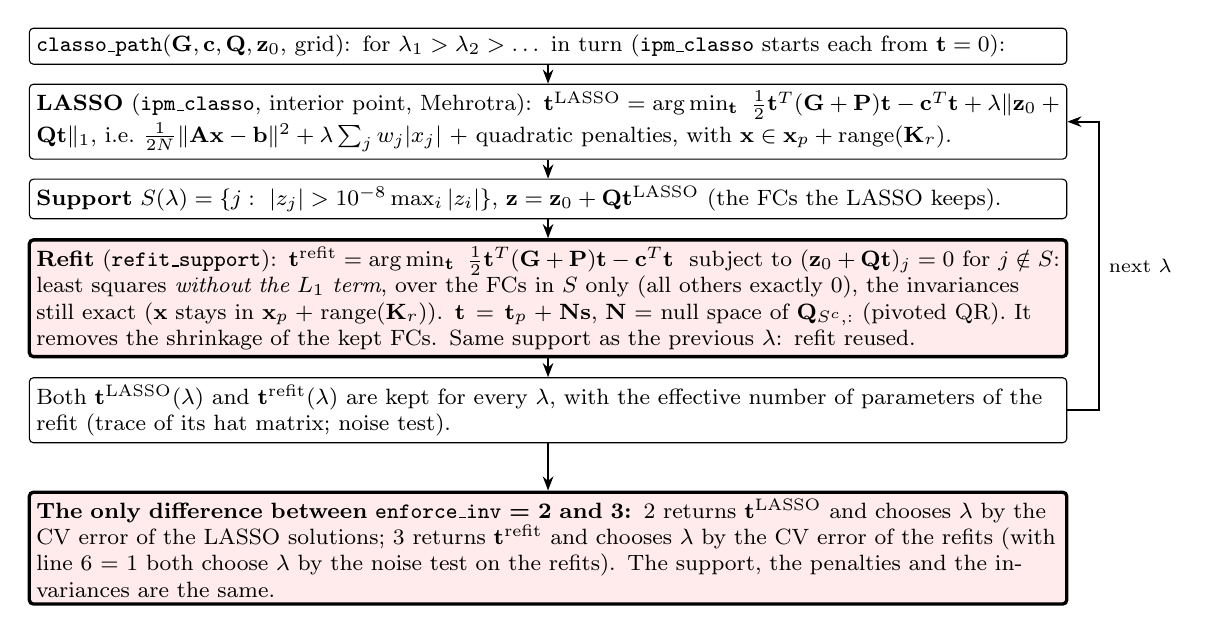
\begin{tikzpicture}[node distance=2.4mm]
\node[box=13cm] (h1) {\code{classo\_path}($\bG,\bc,\bQ,\bz_0$, grid): for $\lambda_1>\lambda_2>\dots$ in turn (\code{ipm\_classo} starts each from $\bt=0$):};
\node[box=13cm, below=of h1] (h2) {\textbf{LASSO} (\code{ipm\_classo}, interior point, Mehrotra):
  $\bt^{\rm LASSO}=\arg\min_\bt\ \tfrac12\bt^T(\bG+\mathbf P)\bt-\bc^T\bt+\lambda\|\bz_0+\bQ\bt\|_1$,
  i.e.\ $\tfrac1{2N}\|\bA\bx-\bb\|^2+\lambda\sum_jw_j|x_j|$ + quadratic penalties, with $\bx\in\bx_p+\mathrm{range}(\bK_r)$.};
\node[box=13cm, below=of h2] (h3) {\textbf{Support} $S(\lambda)=\{j:\ |z_j|>10^{-8}\max_i|z_i|\}$, $\bz=\bz_0+\bQ\bt^{\rm LASSO}$
  (the FCs the LASSO keeps).};
\node[hl=13cm, below=of h3] (h4) {\textbf{Refit} (\code{refit\_support}): $\bt^{\rm refit}=\arg\min_\bt\ \tfrac12\bt^T(\bG+\mathbf P)\bt-\bc^T\bt$
  \ subject to $(\bz_0+\bQ\bt)_j=0$ for $j\notin S$:
  least squares \emph{without the $L_1$ term}, over the FCs in $S$ only (all others exactly 0), the invariances still exact
  ($\bx$ stays in $\bx_p+\mathrm{range}(\bK_r)$). $\bt=\bt_p+\bN\mathbf s$, $\bN$ = null space of $\bQ_{S^c,:}$ (pivoted QR).
  It removes the shrinkage of the kept FCs. Same support as the previous $\lambda$: refit reused.};
\node[box=13cm, below=of h4] (h5) {Both $\bt^{\rm LASSO}(\lambda)$ and $\bt^{\rm refit}(\lambda)$ are kept for every $\lambda$, with the
  effective number of parameters of the refit (trace of its hat matrix; noise test).};
\node[hl=13cm, below=6mm of h5] (h6) {\textbf{The only difference between \code{enforce\_inv} = 2 and 3:} 2 returns $\bt^{\rm LASSO}$ and
  chooses $\lambda$ by the CV error of the LASSO solutions; 3 returns $\bt^{\rm refit}$ and chooses $\lambda$ by the CV error of
  the refits (with line 6 = 1 both choose $\lambda$ by the noise test on the refits). The support, the penalties and the
  invariances are the same.};
\foreach \u/\v in {h1/h2,h2/h3,h3/h4,h4/h5,h5/h6} \draw[arr] (\u) -- (\v);
\draw[arr] (h5.east) -- ++(4mm,0) |- node[pos=0.25,right,font=\scriptsize]{next $\lambda$} (h2.east);
\end{tikzpicture}
\caption{\code{enforce\_inv}=2 and 3, inner level: one LASSO path (\code{lasso\_constrained.f90:classo\_path},
\code{ipm\_classo}, \code{refit\_support}), used on each training set and on all rows. $\mathbf P$: the filter
penalty and, with line 7, the $L_2$ term (the CV training sets use their own Gram matrices with the same
$\mathbf P$).}
\label{fig:lassoinner}
\end{figure}

%==============================================================================
\section{Standard errors for LASSO fits (9.9)}\label{sec:lassoerr}
%==============================================================================
\paragraph{Motivation.} With \code{enforce\_inv}=2, 3 the log printed sd$=0$ (not estimated).

\paragraph{Algorithm.} Take the support $S$ as in Section~\ref{sec:lasso}. The FCs with the invariances
exact and $x_j=0$ off $S$ are $\bx+\bK\bN\bz$, $\bN$ an orthonormal basis of the null space of the rows of
$\bK$ off $S$. The constrained least-squares fit of $\bb-\bA\bx$ on the basis $\bK\bN$ gives the
covariance of Section~\ref{sec:sd}. $\bx$ is not changed. For \code{enforce\_inv}=3 these are the refit's own
errors; for 2 those the refit would have. Neither includes the selection or the shrinkage.

\paragraph{Implementation.} \code{lasso\_support\_errors} (\code{constrained\_fit.f90}), using
\code{null\_space\_qr} (now public) and \code{fit\_kernel\_basis}; file \code{svd-lasso.dat}; log lines
\code{LASSO\_SUPPORT\_ERRORS}. Commit \code{1a13984}.

\paragraph{Validation.} MoTe$_2$: sd(1..3) = $2.8\times10^{-5}$/0.033/142 (\code{enforce\_inv}=0),
$3.0\times10^{-5}$/0.034/62.8 (2), $3.0\times10^{-5}$/0.029/47.8 (3); for 3 this refit reproduces LASSO's refit to
$1.4\times10^{-6}$; FCs byte-identical to 9.8.

%==============================================================================
\section{The smooth SVD filter as a per-mode penalty; the ridge prior (9.9)}\label{sec:filter}
%==============================================================================
\paragraph{Motivation.} The SVD fits (\code{enforce\_inv}=0, 1) damp poorly determined directions with a
smooth filter, while the LASSO cut them with a hard threshold. The four settings should use one
regularization. A Gaussian prior on the FCs was also requested as an option.

\paragraph{Algorithm.} Let $\bA\bK=\sum_kw_k\bu_k\bv_k^T$ and $w_c=c\,w_{\max}$. \code{svbksb} returns
\begin{equation}
\by=\sum_k\frac{w_k^2}{\sqrt{w_k^6+w_c^6}}\,(\bu_k\cdot\bb)\,\bv_k
=\sum_k\frac1{\sqrt{1+(w_c/w_k)^6}}\,\frac{\bu_k\cdot\bb}{w_k}\,\bv_k .
\label{eq:filter}
\end{equation}
The factor $1/\sqrt{1+(w_c/w)^6}$ multiplying the plain inverse is the magnitude response of a
third-order Butterworth filter in the variable $w_c/w$. Below the cut the gain is $w^2/w_c^3$; ridge
regression, $w/(w^2+w_c^2)$, gives $w/w_c^2$. Minimizing $\|\bA\bK\by-\bb\|^2+\sum_kg_k(\bv_k\cdot\by)^2$ gives
$\bv_k\cdot\by=w_k(\bu_k\cdot\bb)/(w_k^2+g_k)$; equating with Eq.~\eqref{eq:filter},
\begin{equation}
g_k=w_k^2\Big(\sqrt{1+(w_c/w_k)^6}-1\Big).
\end{equation}
So the filter is a quadratic penalty with a mode-dependent weight, and it can be added to the LASSO
objective. In the variables of Section~\ref{sec:lasso}, $\by=\mathbf B^{-1}\bt$ with $\mathbf B=\bQ^T\bW\bK_r$, and the
penalty $(1/2N)\sum_kg_ky_k^2$ is $\tfrac12\bt^T\mathbf P\bt$, $\mathbf P=\mathbf B^{-T}\mathrm{diag}(g)\mathbf B^{-1}/N$;
$\bK_r$ holds the right singular directions of $\bA\bK$ with $w_k>10^{-15}w_{\max}$. Without the $L_1$ term the
fit is that of \code{svd\_set}.

\emph{Bayesian reading.} With Gaussian noise of variance $\sigma^2$ and a Gaussian prior of width $\tau$ on each
parameter, the posterior maximum minimizes $\|\bA\bx-\bb\|^2/(2\sigma^2)+\|\bx\|^2/(2\tau^2)$: ridge with
$\lambda_2=\sigma^2/\tau^2$. The filter is the same with a prior width that depends on the mode, $\tau_k^2=\sigma^2/g_k$.

\emph{Optional ridge prior.} With \code{default.params} line 7 = 1 the LASSO objective gets
\begin{equation}
\frac{s^2}N\sum_j\frac{x_j^2}{2\tau_{r(j)}^2},
\end{equation}
with $s^2$ the residual variance of the full filtered least-squares fit and $\tau_r$ the rms of the rank-$r$
FCs of that fit. It enters the LASSO, the refits and the cross-validation training fits; the residuals
(CV errors, noise test) are those of the forces alone.

\paragraph{Implementation.} \code{classo\_cv} (\code{resolved\_kernel} with $10^{-15}$),
\code{classo\_cv\_res} (internal \code{filter\_penalty}; the ridge term with \code{l2fac}, \code{colrank}) in
\code{lasso\_constrained.f90}; switch read in \code{ios.f90} (only the value 1 switches it on; the
environment variable \code{FOCEX\_L2\_TAU} scales $\tau$, for tests only). Commit \code{7f89a43}. The log/
\code{lasso.dat} lines give the number of directions below the filter scale and, with line 7, $s^2$ and $\tau$.

\paragraph{Validation.} ZnO cubic exact model, FC3 to 7 shells while the model has 5, 21\,600 rows, force noise
$10^{-3}$: the run with the hard cut equals the run with the filter (no direction below the filter scale in
these data). Ridge with $\tau\times0.5$, 1, 2: the same within one FC (the term is negligible with these data).
Not tested: noisier data or fewer snapshots.

%==============================================================================
\section{The noise test for the LASSO weight (9.9)}\label{sec:noisetest}
%==============================================================================
\paragraph{Motivation.} Cross-validation chose $\lambda/\lambda_{\max}=1.08\times10^{-4}$ on LaP (FC3 to 6 shells) and kept terms at
the noise level. The weight should follow from the force noise.

\paragraph{Algorithm.} Fit all resolved parameters (filtered least squares): residual $\mathrm{RSS}_{\rm full}$,
effective number of parameters $p_{\rm full}$, and $s^2=\mathrm{RSS}_{\rm full}/(N-p_{\rm full})$. On the
all-rows path, for each $\lambda$ refit on the support and compute $\mathrm{RSS}(\lambda)$ and $p(\lambda)$.
The effective number of parameters is the trace of the hat matrix of the refit,
$p=\Tr[(\bN^T\bG_p\bN)^+\bN^T\bG\bN]$, with $\bG_p$ the Gram matrix including the penalties and $\bG$ that of
the data. With $\Delta p=p_{\rm full}-p(\lambda)$, if the dropped parameters were zero, $\Delta\mathrm{RSS}/s^2$
would be $\chi^2_{\Delta p}$, of mean $\Delta p$ and variance $2\Delta p$. The rule takes the largest $\lambda$ with
\begin{equation}
\mathrm{RSS}(\lambda)-\mathrm{RSS}_{\rm full}\le s^2\big(\Delta p+2\sqrt{2\Delta p}\big)
\end{equation}
(mean plus two standard deviations; a round-off allowance $10^{-13}N\langle b^2\rangle$ is added). With exact
forces $s=0$, and only refits that reproduce the full fit pass. If none passes, the grid is extended as for
the CV.

\paragraph{Implementation.} \code{default.params} line 6 = 1 (\code{lasso\_rule}); \code{classo\_cv\_res},
\code{classo\_path} (argument \code{npf}), \code{refit\_support} (argument \code{pf}) in
\code{lasso\_constrained.f90}. \code{lasso.dat} lists, per $\lambda$, $\mathrm{RSS}-\mathrm{RSS}_{\rm full}$ and the free
parameters, and the line \code{noise test: RSS\_full ... p\_full ... s\^{}2 ... first passing k}.

\paragraph{Validation.} ZnO cubic exact model as above (FC3 to 7 shells, model 5; 229 true FC3).
``LASSO+refit'' is \code{enforce\_inv}=3 with the filter penalty:
\begin{center}
\small
\begin{tabular}{@{}llccccc@{}}
\toprule
forces & method & $\lambda/\lambda_{\max}$ & FC3 $\neq0$ & true lost & false kept & rms err$/\sigma$\\
\midrule
exact & LASSO+refit, noise test & -- & 229 & 0 & 0 & --\\
noise $10^{-3}$ & least squares & -- & 624 & -- & 395 & 0.99\\
noise $10^{-3}$ & LASSO+refit, noise test & $5.4\times10^{-5}$ & 374 & 10 & 155 & 0.64\\
noise $10^{-3}$ & LASSO+refit, CV & $4.2\times10^{-5}$ & 390 & 7 & 168 & 0.62\\
\bottomrule
\end{tabular}
\end{center}
With exact forces FC2 and FC3 are exact ($5.7\times10^{-13}$, $3.3\times10^{-10}$). With noise, $s=0.99\times10^{-3}$
(true $10^{-3}$); the lost terms are all $\le3.2\sigma$ ($\le0.4$\,\% of the largest FC3), the false ones all
$<1.8\sigma$ (median 0.36). About 9\,min and 0.34\,GB per LASSO run. On these data the noise test and CV are close;
data where they differ were not tested.

%==============================================================================
\section{The SVD cut moved into a gap of the singular values (9.9)}\label{sec:gap}
%==============================================================================
\paragraph{Motivation.} The filter of Eq.~\eqref{eq:filter} damps a mode below the cut; it does not remove
it. A nearly singular mode not far below the cut, or just above it, is amplified. In the MgO case of
Section~\ref{sec:ws} this gave FC2 of order $10^5$\,eV/\AA$^2$. Raising the cut just above the small values is
not enough. With line 2 = $4\times10^{-5}$ the relative cut $c=1.6\times10^{-9}$ lies above every small value
($r=1.6\times10^{-10}$), yet FC2 was still 300--500. The gain of that mode below the cut is, in units of
$1/w_{\max}$, $r^2/c^3=6.2\times10^6$; in absolute units ($w=1.87\times10^{-11}$, $w_c=c\,w_{\max}=1.87\times10^{-10}$,
$w_{\max}=0.1167$) $w^2/w_c^3=5.3\times10^7$ per unit of $\bu_k\cdot\bb$, the same number
($6.2\times10^6/0.1167$).

\paragraph{Algorithm.} Let $r_k=w_k/w_{\max}$, sorted ascending, and $c$ the relative cut. A value is
dangerous if
\begin{equation}
\big(r<c\ \text{and}\ r^2>10\,c^3\big)\quad\text{or}\quad c\le r<10^3c .
\end{equation}
Below the cut the gain is $\approx r^2/c^3$; the factor 10 compares it with the gain $1/r$ of a resolved mode
at $r\approx0.1$. Just above the cut the gain is $\approx1/r$. If there is a dangerous value, let $r_{\rm lo}$ be
the largest one; search upward from it for the first gap $r_{k+1}\ge10^3r_k$, and set
\begin{equation}
c\leftarrow r_{\rm lo}^{\,0.1}\,r_{\rm hi}^{\,0.9},
\end{equation}
with $r_{\rm lo}=r_k$, $r_{\rm hi}=r_{k+1}$ the edges of the gap (nearer the good values). Then the top bad mode
has gain $(r_{\rm lo}/r_{\rm hi})^{1.7}/r_{\rm hi}$ and the smallest good mode is changed by
$\tfrac12(r_{\rm lo}/r_{\rm hi})^{0.6}$, at most $8\times10^{-3}$ for a gap of $10^3$ (code comment). Without such a
gap the cut is left unchanged and a message is printed. The cut is never lowered.

\paragraph{Implementation.} Figure~\ref{fig:gap} shows the rule on the sorted singular values.
\code{gap\_cut} (\code{svd\_ridge.f90}), called by \code{svd\_set} and by
\code{classo\_cv\_res} for the LASSO filter. Screen and log: \code{SVD: singular values next to the cut ...;
cut moved to the gap at ...} (or \code{no gap above them: cut unchanged}). The minimum gap was $10^4$ and the new cut the geometric mean of the edges (capped at
$10^{-3}$) in earlier versions of the same day.

\paragraph{Validation.} MgO with Born charges (\code{fc2range}=0, \code{enforce\_inv}=1, 2 single-atom
snapshots): small singular values up to $1.6\times10^{-10}$ of $w_{\max}$, the next $9.1\times10^{-2}$; cut
$1.6\times10^{-9}\to1.21\times10^{-2}$ ($3.82\times10^{-6}$ with the geometric mean; the FCs agree to 4--5 digits); FC2
group 9 from $3.85\times10^5$ to $\le5\times10^{-3}$\,eV/\AA$^2$; fit 0.933\,\% unchanged; largest FC2 11.66. The same
with line 2 = $4\times10^{-5}$. ZnO runs without small values: byte-identical apart from timing.

%------------------------------------------------------------------------------
\begin{figure}[tbp]
\centering
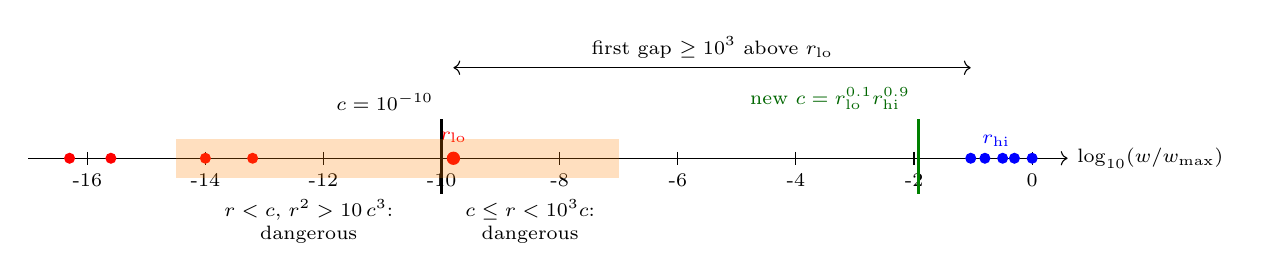
\begin{tikzpicture}[x=0.75cm,y=1cm]
\draw[->] (-17,0) -- (0.6,0) node[right,font=\scriptsize]{$\log_{10}(w/w_{\max})$};
\foreach \e in {-16,-14,...,0} \draw (\e,0.08) -- (\e,-0.08) node[below,font=\scriptsize]{\e};
% round-off modes and the small value
\foreach \e in {-16.3,-15.6,-14.0,-13.2} \fill[red] (\e,0) circle (2pt);
\fill[red] (-9.8,0) circle (2.4pt) node[above=2pt,font=\scriptsize,text=red]{$r_{\rm lo}$};
\foreach \e in {-1.04,-0.8,-0.5,-0.3,0} \fill[blue] (\e,0) circle (2pt);
\node[above right=1pt,font=\scriptsize,text=blue] at (-1.04,0) {$r_{\rm hi}$};
% cut and window
\draw[thick] (-10,-0.45) -- (-10,0.5) node[above left=-1pt,font=\scriptsize]{$c=10^{-10}$};
\fill[orange,opacity=0.25] (-10,-0.25) rectangle (-7,0.25);
\node[font=\scriptsize,align=center] at (-8.5,-0.8) {$c\le r<10^3c$:\\ dangerous};
\fill[orange,opacity=0.25] (-14.5,-0.25) rectangle (-10,0.25);
\node[font=\scriptsize,align=center] at (-12.25,-0.8) {$r<c$, $r^2>10\,c^3$:\\ dangerous};
\draw[<->] (-9.8,1.15) -- node[above,font=\scriptsize]{first gap $\ge10^3$ above $r_{\rm lo}$} (-1.04,1.15);
\draw[very thick,green!50!black] (-1.92,-0.45) -- (-1.92,0.5) node[above left=-1pt,font=\scriptsize,text=green!40!black]{new $c=r_{\rm lo}^{0.1}r_{\rm hi}^{0.9}$};
\end{tikzpicture}
\caption{\code{svd\_ridge.f90:gap\_cut} on the sorted relative singular values, with the MgO numbers of
Section~\ref{sec:gap}: $c=10^{-10}$, $r_{\rm lo}=1.6\times10^{-10}$, $r_{\rm hi}=9.1\times10^{-2}$, new cut
$1.21\times10^{-2}$. Shaded: the dangerous windows; the largest dangerous value, $r_{\rm lo}$, is where the search for
a gap starts. The positions of the round-off values on the left are schematic.}
\label{fig:gap}
\end{figure}

%==============================================================================
\section{Refit when the measured noise exceeds the guess (9.9)}\label{sec:noisecheck}
%==============================================================================
\paragraph{Motivation.} The cut $c=\epsilon_F^2$ comes from the user's guess of the force noise (line 2). If
the forces (or the model) are much noisier, modes below the noise are fitted.

\paragraph{Algorithm.} After the fit, the measured relative noise is
\begin{equation}
\varepsilon^2=\frac{\|\bA\bx-\bb\|^2}{\|\bb\|^2}.
\end{equation}
If $\varepsilon^2>100\,c$ (the measured noise more than 10 times the guess) and $\varepsilon^2$ exceeds the
current cut, the cut is set to $\varepsilon^2$, passed through \code{gap\_cut} (giving $w_c'$), and the
solution is redone from the same SVD. A large misfit can also be model error (missing FCs), not noise; then
a larger cut only removes information. So the refit is kept only if it passes the noise test of
Section~\ref{sec:noisetest}. With the filter factors of \code{svbksb},
\begin{equation}
\phi_k=\frac{w_k^3}{\sqrt{w_k^6+w_c^6}},\qquad p=\sum_k\phi_k ,
\end{equation}
($p$ is the trace of the hat matrix, the effective number of fitted parameters), $s^2=\mathrm{RSS}_{\rm old}/(N-p)$
and $\Delta p=p(w_c)-p(w_c')$, the refit is kept if
\begin{equation}
\mathrm{RSS}_{\rm new}-\mathrm{RSS}_{\rm old}\le s^2\big(\Delta p+2\sqrt{2\Delta p}\big)
\end{equation}
(plus a round-off allowance $10^{-13}\|\bb\|^2$); otherwise the first solution and its errors are kept. The cut
is only raised.

\paragraph{Implementation.} \code{svd\_set} (\code{svd\_ridge.f90}; Fig.~\ref{fig:svdset}; filter factors in its internal function
\code{phif}), active only when the flag \code{svd\_noise\_check} (\code{common/params.f90}) is set.
\code{focex.f90} sets it around the force fits of \code{enforce\_inv}=0 (\code{svd\_set}) and 1
(\code{fit\_kernel\_basis}). It is off for \code{lasso\_support\_errors}: there the fitted vector is a
residual, whose relative misfit is about 1 by construction (running the check there was a bug, found and
fixed on 6 November 2026). The LASSO filter applies the same rule to its full filtered fit
(\code{classo\_cv\_res}, $\varepsilon^2=\mathrm{RSS}/\|\bb\|^2$). Log lines: \code{SVD: measured relative noise
... (line 2 gave ...): refit with the cut ...}, then \code{SVD: refit kept (noise test passed): parameters
dropped ..., RSS increase relative ...} or \code{SVD: refit rejected: ... model error; cut unchanged}.

\paragraph{Validation.} Runs of the final 9.9 build:
\begin{itemize}
\item MgO with Born charges (2 single-atom snapshots, default FC2 range, FC3 3 shells, \code{enforce\_inv}=1).
With the default line 2 ($c=10^{-10}$) the cut moved into the gap (Section~\ref{sec:gap}), and the measured
noise $\varepsilon=1.76\times10^{-3}$ triggered a refit, kept by the test (0.99 parameters dropped, RSS increase
$1.73\times10^{-5}$ relative). The result equals that of the hand-tuned line 2 = $4\times10^{-4}$: fit 0.174\,\% /
0.176\,\%, $\Gamma$ $T_{1u}$ 534.89\,cm$^{-1}$, highest frequency 748.9\,cm$^{-1}$, no unstable $k$, Gr\"uneisen
median (IBZ, $\omega>20$\,cm$^{-1}$) 1.73 / 1.68.
\item MoTe$_2$, FC2 only (the misfit is model error, not noise): first-fit $\varepsilon$ from 0.44 to 0.032 for
2 to 10 FC2 shells; every refit was rejected (10 shells: dropping 8.1 parameters would raise the RSS by a
factor 324). Without the test the refit had taken the misfit for noise and given a 97.8\,\% residual.
\item ZnO cubic exact model: with exact forces no refit, \code{fc3.dat} identical; with $10^{-3}$ noise, refit to
the cut $3.0\times10^{-6}$, FC errors unchanged (FC3 rms 0.99\,$\sigma$).
\end{itemize}

%==============================================================================
\section{Rotational invariants of FC3 and FC4 (9.9)}
%==============================================================================
\paragraph{Motivation.} The range of FC3 and FC4 is to be judged from their size against distance, in a
form that does not depend on the axes.

\paragraph{Algorithm.} For each triplet (quadruplet) of atoms, the Frobenius norm
$\|\Psi\|=(\sum_{\alpha\beta\gamma}\Psi_{\alpha\beta\gamma}^2)^{1/2}$ (likewise $\|\chi\|$), and for FC4 the
isotropic part
\begin{equation}
\mathrm{iso}=\frac13\sum_{\alpha\beta}\big(\chi_{\alpha\alpha\beta\beta}+\chi_{\alpha\beta\alpha\beta}+\chi_{\alpha\beta\beta\alpha}\big),
\end{equation}
both invariant under rotations, against the largest pair distance $d_{\max}$ of the tuple and the number of
distinct atoms. Tuples that differ only by the order of the last indices are written once.

\paragraph{Implementation.} \code{write\_fc\_invariants} (\code{ios.f90}): \code{trace\_fc.dat} blocks 1
(FC3) and 2 (FC4); plotted by \code{FOCEX/PLOTTING/fcs.plt}. Commit \code{1a13984}.

\paragraph{Validation.} MoTe$_2$: 506 triplets, norms equal to a Python recomputation from \code{fc3.dat} to
$3\times10^{-5}$ (rounding). The FC4 plot branch was tested for gnuplot syntax only.

%==============================================================================
\section{Wigner--Seitz boundary aliasing}\label{sec:ws}
%==============================================================================
\paragraph{Problem.} In a supercell with lattice $\{L\}$, a displacement of atom $j$ moves all its images. The
force on atom $i$ sees $\sum_L\Phi(i,j+L)$. If a pair $(i,j)$ has several images at the same distance on the
boundary of the supercell Wigner--Seitz cell, the data fix only their sum. With $d_k$ the image vectors
related by point operations $R_k$ ($\Phi(d_k)=R_k\Phi(d_1)R_k^T$), the data see
\begin{equation}
\Phi(d_1)\ \mapsto\ \sum_kR_k\,\Phi(d_1)\,R_k^T ,
\end{equation}
restricted to the components that the site symmetry of $d_1$ allows. Combinations in the kernel of this map
are invisible to any data of this supercell; equal weights of the images do not change the rank.

\paragraph{MgO case.} Run with Born charges, \code{fc2range}=0 (whole supercell), \code{enforce\_inv}=1, 2
single-atom snapshots of 0.0106\,\AA. FC2 group 9 (Mg--O at 6.991\,\AA) came out at $\pm10^5$\,eV/\AA$^2$ (385136,
$-208352$, \dots), sd(2) $9.7\times10^4$, Hill $B$ printed as $-4\times10^7$. The pair lies on the boundary of the
4$\times$4$\times$4 rhombohedral supercell: three images $v_1=(-\tfrac32,-\tfrac12,-\tfrac12)$,
$v_2=(\tfrac12,-\tfrac12,\tfrac32)$, $v_3=(\tfrac12,\tfrac32,-\tfrac12)$ (units of the cubic $a$), all at
$a\sqrt{5.5}=6.991$\,\AA. The site group of $v_1$ has order 2, leaving 5 components. The image-sum map has
singular values 3, 3, 0, 0, 0: rank 2 of 5. Three combinations are invisible. Their singular values in
\code{svd-kernel.dat} were round-off (5$\times10^{-17}$ to $1.5\times10^{-14}$, with $w_c=1.17\times10^{-11}$). The filter gain
$w^2/w_c^3$ (absolute, per unit of $\bu_k\cdot\bb$) is $1.3\times10^5$ at $w=1.45\times10^{-14}$ (ridge would give
$w/w_c^2\approx10^8$, a hard cut 0); hence FC2
$\pm10^5$. The same gain arises in the LASSO filter. The earlier runs with \code{fc2range}=1 (6 shells) were fine:
largest FC2 11.66, fit 2.02\,\% (Born), 7.20\,\% (no Born).

\paragraph{Remedy and open points.} The gap rule of Section~\ref{sec:gap} moves the cut above these modes and
gives FC2 of group 9 $\le5\times10^{-3}$\,eV/\AA$^2$. Proposed, not done: zero modes below a round-off level
(about $10^{-13}w_{\max}$), or keep only the visible combination of boundary FC2 groups (or drop
rank-deficient boundary groups). Not checked in the code: why the keep rule kept group 9. A related case was
recorded in 9.1: on a ZnO 3$\times$3$\times$2 supercell, groups at 5.0--6.0\,\AA{} lie wholly on the boundary, only
$\Phi(d)+\Phi(d+L)$ is fixed, the FCs are off by 0.1 and the bands by 11.8\,cm$^{-1}$, exact only at the
commensurate $k$; a 4$\times$3$\times$2 supercell with the same shortest vector gives every FC2 exactly.

%==============================================================================
\section{\texorpdfstring{Invariances with an inconsistent model: MoTe$_2$}{Invariances with an inconsistent model: MoTe2}}\label{sec:mote2}
%==============================================================================
\paragraph{Motivation.} FOCEX never gave good results for 2H-MoTe$_2$: unstable interlayer modes and
negative elastic constants. MoTe$_2$ is a layered crystal whose interlayer forces are weak. A small
inconsistency between the data, the truncated model and an imposed invariance then lands in the soft
interlayer FCs. This section separates the causes. System: 6 atoms per cell, 4$\times$4$\times$2 supercell of 192
atoms. \code{FORCEDISP1}: the reference and 6 single-atom snapshots; \code{FORCEDISP2}: 33 single-atom and 376
pair snapshots, pair distances 2.705--9.257\,\AA. All runs with the 9.9 build on 6 November 2026.

\subsection{Data consistency check}
\paragraph{Algorithm.} Forces are short-ranged after subtraction of the reference forces. For each snapshot
$s$ with displaced atoms $D_s$ take the far atoms
$\mathcal F_s=\{i:\min_{j\in D_s}|X_i-X_j|>R_{\rm far}\}$ and compute
\begin{equation}
\delta_s=\Big[\frac1{3|\mathcal F_s|}\sum_{i\in\mathcal F_s}\big|F_i^{(s)}-F_i^{\rm ref}\big|^2\Big]^{1/2} .
\end{equation}
In a consistent data set $\delta_s$ is at the noise level. A snapshot with a large $\delta_s$ was computed
with a different reference (other settings, unconverged, other structure).

\paragraph{Result.} $R_{\rm far}=9$\,\AA. \code{FORCEDISP1} snapshots 2--4 (displacement 0.0100\,\AA) give
$\delta=1.7\times10^{-3}$\,eV/\AA, with far forces about 0, while the reference has Te forces $\pm4.906\times10^{-3}$\,eV/\AA{}
along $z$. Snapshots 5--7, and 402 of the 409 \code{FORCEDISP2} snapshots, agree to $<2\times10^{-4}$\,eV/\AA{}
(median $4\times10^{-5}$). Without snapshots 2--4 the FC2-only fit with 10 shells goes from 12.7\,\% to 3.2\,\%. This
check is recommended as a data diagnostic; it is not part of FOCEX.

\subsection{Prediction of snapshots not used in the fit}
Fit: FC2 10 shells, FC3 2 shells, invariances \code{1 0 0 1}, on the 413 consistent snapshots. Then the forces of the 7
\code{FORCEDISP1} snapshots are predicted with
\begin{equation}
F_I=-\Pi(I)-\sum_J\Phi(I,J)\,u_J-\tfrac12\sum_{JK}\Psi(I,J,K)\,u_Ju_K ,
\end{equation}
using only terms whose first atom is in the primitive cell, with the images folded into the supercell (the formulas of
ANFOMOD's \code{calculate\_potential}, \code{anfomod.f90} lines 183--243, checked by reading). Relative errors: the reference
0.17\,\%, snapshots 5--7 0.83--1.00\,\% (fit error 0.84\,\%); the three inconsistent snapshots 2--4 29.2, 30.3, 18.2\,\%
(rms $1.72\times10^{-3}$\,eV/\AA). Predicted without FC1, snapshots 2--4 give 10.3, 10.7, 6.5\,\% (rms $6\times10^{-4}$) while the
consistent snapshots then give 30--33\,\%. So about two thirds of their discrepancy is that they show none of the
reference's residual forces at the same geometry (other DFT settings; the cause is not known: the data came from
another person's calculations). These snapshots were removed from \code{MoTe2/FORCEDISP1} and \code{MoTe2/TEST/FORCEDISP1}
(originals kept as \code{FORCEDISP1.with\_snaps2-4}); the remaining \code{FORCEDISP1} snapshots displace only Te, so
\code{FORCEDISP1} alone no longer fixes the Mo FC2.

\paragraph{Recommended data diagnostics.} (1) The far-atom check above: forces on atoms far from every displaced atom
must equal the reference forces. (2) A held-out prediction: fit without some snapshots and predict their forces; a
prediction error far above the fit error flags inconsistent data or a model that is too short.

\subsection{Huang rows with zero stress at a reference out of equilibrium}
Without \code{stress.params} the Huang rows impose Eq.~\eqref{eq:huang} with $\sigma=0$, but this reference
is not at equilibrium (Te forces above). FC2 to 10 shells, \code{enforce\_inv}=1: interlayer shear mode
$E_{2g}^2=-64.8$\,cm$^{-1}$, 93 unstable $k$-points on the path, fit 3.23\,\%. With \code{ihuang}=0:
$E_{2g}^2=+26.3$\,cm$^{-1}$, none unstable, fit 1.63\,\%. \code{enforce\_inv}=0 (Huang rows only fitted):
$+27.6$\,cm$^{-1}$.

\subsection{FC2 range}
With \code{ihuang}=0 and the single-atom data:
\begin{center}
\small
\begin{tabular}{@{}lcccccc@{}}
\toprule
FC2 shells & 4 & 6 & 8 & 10 & 12 & 14\\
\midrule
fit (\%) & 5.65 & 3.04 & 2.35 & 1.63 & 1.60 & 1.55\\
$E_{2g}^2$ (cm$^{-1}$) & 39.0 & 22.4 & 25.3 & 26.3 & 25.5 & 25.3\\
\bottomrule
\end{tabular}
\end{center}
10 shells were chosen. The elastic constants are then (GPa) $C_{11}$ 150.3, $C_{12}$ 92.9, $C_{13}$ 15.6, $C_{33}$
46.4, $C_{44}$ 25.0, $C_{66}$ 28.7. The default FC2 range (\code{fc2range}=0) stops in \code{force\_constants}
(atom not found): it needs a larger neighbour search (\code{default.params} line 3).

\subsection{Rotational invariance with truncated FC3}
All 413 consistent snapshots, FC2 to 10 shells, \code{ihuang}=0, \code{enforce\_inv}=1:
\begin{center}
\small
\begin{tabular}{@{}lccccc@{}}
\toprule
FC3 shells, \code{irot} & fit (\%) & $B_{1g}$ (cm$^{-1}$) & unstable $k$ & $C_{33}$ (GPa) & Gr\"uneisen\\
\midrule
2, \code{irot}=1 & 2.79 & $-29.2$ & 74 & $-30.3$ & $-7.9$..0.7, median $-0.09$\\
3, \code{irot}=1 & 1.24 & 28.9 & 0 & 28.2 & --\\
2 or 3, \code{irot}=0 & 0.84 & 37.3 & 0 & 45.7 & 0.0..1.08, median 0.60\\
\bottomrule
\end{tabular}
\end{center}
$B_{1g}$ is the breathing mode. \code{enforce\_inv}=0 with 2 FC3 shells and \code{irot}=1 gives the same as
\code{enforce\_inv}=1 ($B_{1g}$ $-29.1$\,cm$^{-1}$, $C_{33}$ $-30.1$\,GPa). With \code{irot}=0 the results for 2 and 3 FC3
shells are identical: $E_{2g}^2$ 26.3\,cm$^{-1}$; $C_{11}$ 118.3, $C_{12}$ 18.0, $C_{13}$ 13.9, $C_{33}$ 45.7, $C_{44}$ 26.5,
$C_{66}$ 50.2 ($=(C_{11}-C_{12})/2$) GPa; long-wave $C_{11}$ 118.4, $C_{33}$ 45.7, $C_{44}$ 23.1\,GPa. FC3: 102
independent, 97 of them above $2\sigma$.

\paragraph{Interpretation (not proven).} The rank-3 rotational relations of Section~\ref{sec:invrows} tie FC2 to
FC3. With FC3 truncated far shorter than FC2 (2--3 shells against 10) they cannot hold for the true FCs, and
imposing them distorts the soft interlayer FC2.

\subsection{Relaxation}
\code{default.params} line 5 = 1 on the \code{irot}=0 fit (no \code{stress.params}: the reference stress from
FC1): Te moved by $\pm2.257\times10^{-4}$\,\AA{} along $z$, consistent with force over stiffness
($4.906\times10^{-3}/2.257\times10^{-4}=21.7$\,eV/\AA$^2$); strain $-1.19\times10^{-4}$ in plane and $+1.58\times10^{-4}$ along
$c$; largest stress after relaxation $1.4\times10^{-12}$\,GPa; 97\,s. The $\Gamma$ modes change by less than
0.05\,cm$^{-1}$; the $C_{ij}$ are unchanged.

\paragraph{Lessons.} For MoTe$_2$ the problems came from the inputs and the constraints, not from the fitting
algorithm (see also Section~\ref{sec:invfit}): three inconsistent snapshots, Huang rows with $\sigma=0$ at a reference out of equilibrium, and
rotational rows of rank 3 with FC3 truncated short. Check the data first (far-atom forces); give the reference
stress, or switch the Huang rows off; switch the rotational rows off when FC3 is much shorter than FC2.

%==============================================================================
\section{Code audit of 6--7 November 2026}\label{sec:audit}
%==============================================================================
An audit of the solver paths (Section~\ref{sec:inhom}, Figs.~\ref{fig:linsys}--\ref{fig:lassoinner}) found and fixed:
\begin{itemize}
\item \code{itemp}=1 projected the Boltzmann-weighted solution on the kernel without the particular solution, so it
gave $\bC\bx=0$ instead of $\bC\bx=\bd$ (wrong with \code{stress.params}, \code{include\_fc}=2 or \code{born\_flag}=2). Now
$\bx=\bx_p+\bK\bK^T(\bx_{\rm out}-\bx_p)$ (\code{focex.f90}, \code{itemp} branch). Not run: there is no \code{itemp}=1 test case.
\item With no invariance rows (\code{itrans}=\code{irot}=\code{ihuang}=0) and \code{enforce\_inv}$\ge1$ the SVD of an empty matrix
gave an empty kernel and all FCs zero. Now $\bK$ = identity. Checked: MoTe$_2$ FC2-only with \code{0 0 0 1}: fit 1.614\,\%
with non-zero FCs.
\item $\max|\bC\bx_p-\bd|$ was only logged. Now a WARNING if it exceeds $10^{-6}\max|\bd|+10^{-8}$. The absolute floor is
needed: the Coulomb right-hand sides of MgO are round-off (about $5\times10^{-15}$).
\item The violation tables of the log now all print row, $\bC\bx-\bd$ and $\bd$ (the translational table printed $\bC\bx$
without $\bd$, wrong with \code{include\_fc}=2; the rotational one printed $\bC\bx$ and $\bd$).
\end{itemize}
Regression: ZnO cubic exact model (exact and noisy forces): \code{fc2.dat}, \code{fc3.dat} byte-identical; MgO with Born
charges: identical results.

\paragraph{Relative symmetry tests (7 November 2026).} The symmetry tests on matrices built from the fitted FCs are now
relative: a matrix $A$ fails if $\max|A-A^T|>10^{-6}\max|A|$ (antisymmetry likewise). This applies to
\code{dynamical.f90:get\_phi\_zeta\_Xi} ($\Phi$ and $\Gamma$ symmetric, each $\zeta(:,:,\lambda)$ antisymmetric; these stop the
run), \code{extratools.f90:check\_herm\_sym\_R} and \code{check\_herm\_sym\_G} (were $10^{-8}$ absolute) and the warning of
\code{common/linalgb.f90:symmetrize2} (was $10^{-4}$ absolute); \code{make\_hermitian} was already relative ($10^{-6}$).
A matrix that vanishes by symmetry needs a physical scale instead of its own largest element, which is then round-off:
$\zeta=\sum\Phi R$ and $\Gamma=\sum\Phi RR$ are tested against $10^{-6}\max(\max|\zeta|\ \text{or}\ \max|\Gamma|,\ \max|\Phi|)$.
With the purely relative test, MgO ($\zeta=0$ by inversion symmetry, entries $\sim10^{-15}$) stopped at ``Zeta NOT
ANTISYMMETRIC''. The
absolute test $10^{-12}$ on the squared differences had stopped a badly fitted MoTe$_2$ model, with entries of about
$6\times10^5$, at ``GAMA NOT SYMMETRIC'' on round-off. That case (FC2 with 2 or 3 shells, Huang rows on) now runs to the end
and is reported normally: fit 25.8\,\%, a useless model, which the fit error and the phonons show.

\paragraph{Remaining (not fixed).}
\begin{itemize}
\item The removal of repeated rows (\code{compare2previous\_lines}, called in \code{gather\_rows}) compares only the
coefficients of the fitted columns, not the right-hand sides.
\item \code{born\_flag} 3--9 subtract a Coulomb force but give the rotational and Huang rows no right-hand side.
\item Read FCs are not checked against the reference structure of the run that wrote them (the old positions are read
but not compared).
\end{itemize}

%==============================================================================
\section{Invariances and the fit error}\label{sec:invfit}
%==============================================================================
Adding an exact constraint to a least-squares problem can never lower its residual on the fitted data: the
constrained minimum is taken over a subset of the unconstrained one (for the plain least-squares problem; the
regularization filter of Section~\ref{sec:filter} is small where the data resolve the FCs). A constraint can lower the
error on data \emph{not} used in the fit: less noise is fitted and the model is more physical. Hence the diagnostic:
a small increase of the fit error when an invariance is imposed is normal; a large one means that the model is
inconsistent with that invariance. Typical causes: ranges or ranks too short; a wrong (or missing) reference stress;
Born charges and dielectric tensor inconsistent with the supercell calculations (DFPT must use the same functional,
pseudopotentials, cutoff energy and a commensurate $k$-mesh as the supercell runs).

MoTe$_2$ (Section~\ref{sec:mote2}) shows both cases. Imposing the Huang rows with $\sigma=0$ at a reference out of
equilibrium raised the fit error from 1.63\,\% to 3.23\,\% and made the shear mode unstable: the model (zero stress) is
inconsistent with the data. Imposing the rotational rows with FC3 truncated to 2 shells raised it from 0.84\,\% to
2.79\,\% with unstable modes, and with 3 FC3 shells from 0.84\,\% to 1.24\,\% with stable modes: the inconsistency shrinks as
the FC3 range grows.

%==============================================================================
\section{Shell selection tool: \code{shell-optimizer}}\label{sec:shellopt}
%==============================================================================
\paragraph{Motivation.} The FC2 and FC3 ranges are set by numbers of neighbour shells per atom
(\code{structure.params} lines 13, 14). The MoTe$_2$ study (Section~\ref{sec:mote2}) shows how much the results depend
on them, and choosing them by hand takes many runs. Two observations shaped the tool. First, with pair (or random)
snapshots an FC2-only fit absorbs the FC3 part of the forces: in an earlier run of the tool its FC2 changed with
the range so much that $C_{11}$ jumped between 54 and 153\,GPa from one radius to the next. So when FC3 is requested
the FC2 loop already carries a short FC3. Second, the fit error and the dispersion barely depend on the FC3 range,
so they cannot decide it; the FC3 range is chosen from the data support instead (how many of the added FC3 the
data determine).

\paragraph{Algorithm} (\code{FOCEX/utility/shell-optimizer DIR}, Python, standard library only; read from the current
file; its docstring still describes an older FC2 loop without FC3):
\begin{enumerate}
\item Probe: one FOCEX run on the first snapshot only (FC2, 2 shells) gives, from the log, the neighbour shells of every
atom of the primitive cell (radius, number of neighbours).
\item Candidate radii: the middles of the gaps between consecutive shells whose relative size is at least \code{--gap}
(default 0.08), over all atoms, each converted to a number of shells per atom; radii giving the same shell set are
merged.
\item FC2 loop over up to \code{--nfc2} radii (default 6; the smallest candidate is skipped when there are more than
\code{--nfc2}). With FC3 requested (\code{--nfc3} $>0$) ranks 1--3 are fitted with FC3 fixed at the smallest candidate
radius; otherwise ranks 1--2. Recorded: fit error, unstable $k$-points on the band path, lowest frequency, largest
change of the dispersion to the next radius, lowest $\Gamma$ modes, elastic constants. Overflowed output fields
(\code{*****}) and NaN count as infinite (\code{fnum}).
\item FC2 choice (\code{choose}): the smallest radius whose phonons are stable, whose fit error is within \code{--tol-fit}
(default 0.15 percentage points) of the best stable one, and whose dispersion changes by less than \code{--tol-freq}
(default 2\,cm$^{-1}$) to the next radius; if none qualifies, the stable run with the smallest fit error. A warning is
printed if the largest radius tried is chosen.
\item If no FC2 radius is stable: the best-fitting radius is rerun with the Huang rows off, the rotational rows off,
and both off (those that are on); the first setting with stable phonons is taken, and the FC2 loop is redone with it.
\item FC3 loop (ranks 1--3, FC2 as chosen) over up to \code{--nfc3} radii (default 3) not beyond the FC2 radius. Recorded:
fit error, unstable $k$, dispersion change, the Gr\"uneisen parameters (IBZ, $\omega>20$\,cm$^{-1}$) as 1st percentile,
median and 99th percentile, and the number of FC3 above twice their standard error.
\item FC3 choice by data support (\code{choose\_fc3}): among the models with stable phonons and Gr\"uneisen 1\,\%--99\,\% within
$\pm10$, start at the smallest radius and go to the next one as long as at least 25\,\% of the FC3 it adds exceed twice
their standard error.
\item Invariance check on the chosen model: rerun with the rotational rows off and with the Huang rows off (those that
are on); an invariance is flagged if the fit error falls below 0.7 of its value or unstable phonons become stable
(Section~\ref{sec:invfit}). If one is flagged, the FC3 loop is redone with it off (FC2 shells kept).
\item Report \code{DIR/shellopt/report.txt}: the tables and the recommended line 5 and lines 12--14 of
\code{structure.params}.
\end{enumerate}

\paragraph{Validation: MoTe$_2$.} Consistent data (\code{FORCEDISP1} without snapshots 2--4, and \code{FORCEDISP2}: 413
snapshots), started from the author's invariances \code{1 1 1 1}, options \code{--gap 0.05 --nfc2 9 --nfc3 3}. The run used
the build before the FC3 data-support rule; that rule was then applied to the same run directories with
\code{choose\_fc3}.
\begin{itemize}
\item With \code{1 1 1 1} no FC2 radius was stable (e.g.\ 9.83\,\AA: fit 2.275\,\%, 203 unstable $k$). At 9.83\,\AA: Huang off
2.269\,\%, 9 unstable; rotational off 1.556\,\%, 81 unstable; both off 0.620\,\%, 0 unstable. The tool continued with
\code{1 0 0 1}.
\item FC2 loop with \code{1 0 0 1} (FC3 fixed at 3.10\,\AA), all radii stable:
\begin{center}
\small
\begin{tabular}{@{}lccccccccc@{}}
\toprule
$R$ (\AA) & 3.80 & 4.21 & 4.72 & 5.45 & 5.85 & 6.66 & 7.76 & 8.52 & 9.83\\
\midrule
fit (\%) & 4.824 & 4.527 & 3.597 & 2.636 & 1.927 & 1.454 & 0.752 & 0.647 & 0.620\\
$\Delta\omega$ to next (cm$^{-1}$) & 43.98 & 6.00 & 17.14 & 9.31 & 17.16 & 4.11 & 2.57 & 1.53 & --\\
\bottomrule
\end{tabular}
\end{center}
Chosen 8.52\,\AA{} (shells 13 13 21 21 21 21): $C_{11}$ 115.9, $C_{12}$ 26.2, $C_{13}$ 11.5, $C_{33}$ 44.2, $C_{44}$ 24.9,
$C_{66}$ 44.8\,GPa; lowest $\Gamma$ modes 25.6 (shear), 36.6 (breathing), 119.1, 120.9\,cm$^{-1}$.
\item FC3 loop:
\begin{center}
\small
\begin{tabular}{@{}lccc@{}}
\toprule
$R$ (\AA) & 3.10 & 3.80 & 4.21\\
\midrule
fit (\%) & 0.647 & 0.614 & 0.612\\
Gr\"uneisen (1\,\%, median, 99\,\%) & $(-0.68, 0.17, 0.58)$ & $(-0.28, 0.61, 1.30)$ & $(0.10, 0.83, 7.25)$\\
FC3 $>2\sigma$ & 24/24 & 77/140 & 80/179\\
\bottomrule
\end{tabular}
\end{center}
The former rule (fit within tolerance) picked 3.10\,\AA. The data-support rule picks 3.80\,\AA{} (shells 2 2 3 3 3 3): the
116 FC3 added at 3.80\,\AA{} have 53 above $2\sigma$, the 39 added at 4.21\,\AA{} only 3. The Gr\"uneisen median 0.61 agrees
with the hand-chosen model of Section~\ref{sec:mote2} (FC2 10 shells, FC3 2 shells: median 0.60).
\item Recommended: line 5 = \code{1 0 0 1}; FC2 shells 13 13 21 21 21 21; FC3 shells 2 2 3 3 3 3.
\end{itemize}

%==============================================================================
\section{Conclusions}
%==============================================================================
Versions 9.0--9.9 changed three things in FOCEX. First, the constraints: invariance rows of all ranks are
built in one loop, the Huang rows hold for a stressed reference, the structure and tensors are symmetrized,
and the Coulomb part of \code{born\_flag}=2 enters the rows consistently. Second, the physics after the fit:
elastic constants by Born--Huang and by long waves, $B_0'$ from FC3, a quasi-harmonic model with $B_T$ and
$d\ln L/dT$, Gr\"uneisen parameters with an exact $\Gamma$ limit, a relaxation that is exact on the test
models (with point charges through the full Ewald energy), and symmetry labels of the $\Gamma$ modes. Third,
the fit itself: standard errors, a constrained LASSO with exact invariances, and in 9.9 one regularization
for all settings (the smooth filter as a penalty), a noise-based choice of $\lambda$, and rules that protect the
fit against nearly singular modes and against misfit that is model error. The MoTe$_2$ study shows that, for
a soft layered crystal, inconsistent data and invariances imposed on a truncated or out-of-equilibrium
model matter more than the fitting method. Table~\ref{tab:summary} lists the changes.

\paragraph{Open points recorded in the sources.}
\begin{itemize}
\item The data consistency checks of Section~\ref{sec:mote2} (far-atom forces, held-out prediction) are not part of FOCEX.
\item From the audit (Section~\ref{sec:audit}): duplicate-row removal ignores the right-hand sides; \code{born\_flag} 3--9
have no Coulomb right-hand sides; read FCs are not checked against the reference of the run that wrote them;
the \code{itemp}=1 fix is not tested.
\item MoTe$_2$: the explanation of the rank-3 rotational rows is an interpretation, not proven.
\item Noise test and ridge prior: tested only on one exact model with $10^{-3}$ noise; noisier data or fewer
snapshots not tested.
\item Wigner--Seitz boundary groups: the gap rule treats the symptom; removing the invisible combinations is
proposed, not done.
\item Anisotropic $Z^*$: the relaxation keeps the second-order Coulomb route; the rank-4 rotational right-hand
side for tensor $\epsilon$ is not implemented.
\item The FC3 standard errors are 10--15\,\% larger than the observed errors on the exact model; cause unknown.
\item Rotational rows raise the held-out force error in cross-validation on GaN and ZnO (recorded at 9.6);
cause open.
\item ZnO long-wave $C_{33}$ 45--49\,GPa in every setting, against about 210 measured (recorded at 9.6).
\end{itemize}

\begin{table}[t]
\centering
\caption{Summary of the changes. ``Switch'' is the input that turns a change on, if any.}
\label{tab:summary}
\small
\begin{tabular}{@{}lp{7.6cm}p{4.6cm}@{}}
\toprule
Version & Change & Switch\\
\midrule
9.0 & Invariance rows of all ranks in one loop; rotational offsets fixed & --\\
9.0 & $Z^*$, $\epsilon$ checked against the space group & \code{born\_flag}$\neq0$\\
(9.1 tag)$^a$ & Range of FC3--FC8 clusters & \code{structure.params} l.\,12 flags\\
(9.1 tag)$^a$ & Generalized Huang rows, stressed reference & \code{stress.params}; Huang flag\\
(9.1 tag)$^a$ & Constrained LASSO, exact invariances, refit & \code{enforce\_inv}=2, 3\\
9.1 & Frequencies at the exact $k$; $\Gamma$ as a limit & --\\
9.2 & Born--Huang elastic constants; $B_0'$ from FC3; QHA with $B_T$, $d\ln L/dT$ & --\\
9.2 & Mode Gr\"uneisen parameters at $k$, long-wave limit at $\Gamma$ & --\\
9.2 & Standard errors sd(rank) & --\\
9.3 & Relaxation of an unrelaxed reference & \code{default.params} l.\,5 = 1\\
9.4 & IR/Raman activity, irreps, computed character tables; \code{tol\_sym}; $\Gamma$ threshold & --\\
9.5 & Some ranks read, others fitted & \code{include\_fc}=2\\
9.5 & Hybrid Coulomb subtraction, Coulomb right-hand sides & \code{born\_flag}=2\\
9.5 & Elastic constants from long-wave sound speeds & --\\
9.5 & Irreducible wedge from the Laue group (shared) & --\\
9.6 & Symmetrized positions, $Z^*$, $\epsilon$, stress & --\\
9.7 & OpenMP SVDs, \code{-O3}, identical results & \code{FOCEX\_NUM\_THREADS}\\
9.7 & Coulomb FCs (second order) in the relaxation & \code{born\_flag}=2, l.\,5 = 1\\
9.8 & Exact Coulomb relaxation by Broyden; relax-only reruns & $Z^*=z\mathbb 1$; all \code{include\_fc}=2\\
9.9 & Standard errors for LASSO fits & \code{enforce\_inv}=2, 3\\
9.9 & SVD filter as per-mode penalty in the LASSO & \code{enforce\_inv}=2, 3\\
9.9 & Noise test for $\lambda$ & \code{default.params} l.\,6 = 1\\
9.9 & Ridge prior, $\tau$ = rms per rank & \code{default.params} l.\,7 = 1\\
9.9 & SVD cut moved into a singular-value gap & --\\
9.9 & Refit when measured noise $>100\times$(l.\,2)$^2$, kept if it passes the noise test & -- (force fits)\\
9.9 & FC3/FC4 invariants in \code{trace\_fc.dat} & --\\
9.9 & Audit fixes: $\bx_p$ in \code{itemp}=1, $\bK=1$ without rows, \code{presid} warning, violation tables & --\\
9.9 & \code{shell-optimizer} (FC2/FC3 shell selection; FC3 range from data support) & \code{FOCEX/utility}\\
9.9 & Relative symmetry tests ($10^{-6}\max|A|$) in \code{get\_phi\_zeta\_Xi}, \code{check\_herm\_sym}, \code{symmetrize2} & --\\
\bottomrule
\end{tabular}

\smallskip
\raggedright\footnotesize
$^a$ Commit \code{c9edf0a}, 27 October 2026: after the 9.0 tag, inside the 9.1 tag; not in the manual's history.
\end{table}

\end{document}
